\documentclass[11pt,a4paper]{article}
\usepackage{lmodern}
\usepackage{fontspec}
\setmainfont{LibreBaskerville}[Path=fonts/,Extension=.ttf,UprightFont=*-Regular,BoldFont=*-Bold,ItalicFont=*-Italic,BoldItalicFont=*-BoldItalic,Ligatures=TeX]
\setmonofont{lmmono10-regular.otf}[Scale=0.88]
\usepackage[a4paper,margin=18mm,headheight=16pt,headsep=8mm,footskip=10mm]{geometry}
\usepackage{microtype,amsmath,amssymb,graphicx,booktabs,tabularx,array}
\usepackage[table]{xcolor}
\usepackage{enumitem,fancyhdr,titlesec,tikz,caption,float,listings,setspace}
\usetikzlibrary{arrows.meta,positioning}
\usepackage[hidelinks]{hyperref}
\definecolor{accent}{HTML}{12636A}
\definecolor{ink}{HTML}{24343D}
\definecolor{light}{HTML}{EDF4F3}
\definecolor{orange}{HTML}{B85D17}
\setlength{\parindent}{0pt}
\setlength{\parskip}{4pt}
\onehalfspacing
\renewcommand{\arraystretch}{1.15}
\setlength{\tabcolsep}{4pt}
\setlist{nosep,leftmargin=1.5em}
\setlist[enumerate]{itemsep=3pt}
\raggedbottom
\clubpenalty=10000\widowpenalty=10000
\titleformat{\section}{\fontsize{17}{21}\selectfont\bfseries\color{black}}{\thesection}{0.6em}{}
\titleformat{\subsection}{\normalsize\bfseries\color{black}}{}{0em}{}
\titlespacing*{\section}{0pt}{4pt}{7pt}
\titlespacing*{\subsection}{0pt}{8pt}{3pt}
\captionsetup{font=small,labelfont=bf,skip=4pt,justification=raggedright,singlelinecheck=false}
\setlength{\intextsep}{7pt}
\pagestyle{fancy}\fancyhf{}
\fancyhead[L]{\fontsize{8.5}{10}\selectfont OpenGL Conveyor Box Sorting System}
\fancyhead[R]{\fontsize{8.5}{10}\selectfont CSE 4102}
\fancyfoot[C]{\small\thepage}
\renewcommand{\headrulewidth}{0.3pt}
\newcolumntype{Y}{>{\raggedright\arraybackslash}X}
\newcolumntype{L}[1]{>{\raggedright\arraybackslash}p{#1}}
\newcommand{\code}[1]{{\urlstyle{tt}\nolinkurl{#1}}}
\newcommand{\source}[1]{\par{\fontsize{8.5}{11}\selectfont\raggedright\textbf{Implementation:} #1\par}}
\newcommand{\note}[1]{\par\noindent #1\par}
\newcommand{\implemented}{\textbf{Implemented}}
\newcommand{\adapted}{\textbf{Adapted}}
\newenvironment{shot}[3][\linewidth]{\def\shotcaption{#3}\begin{figure}[H]\centering\begin{tikzpicture}\node[anchor=south west,inner sep=0] (shot) at (0,0) {\includegraphics[width=#1]{#2}};\begin{scope}[x={(shot.south east)},y={(shot.north west)}]}{\end{scope}\end{tikzpicture}\caption{\shotcaption}\end{figure}}
\newcommand{\callout}[3]{\draw[white,line width=2.2pt] (#2)--(#1);\draw[accent,line width=0.75pt,-{Latex[length=1.8mm]}] (#2)--(#1);\node[fill=white,draw=accent,rounded corners=1pt,inner sep=3pt,font=\fontsize{8}{10}\selectfont\bfseries,text=ink] at (#2) {#3};}
\lstset{basicstyle=\ttfamily\small,breaklines=true,columns=fullflexible,keepspaces=true,frame=single,rulecolor=\color{accent!30},backgroundcolor=\color{light},showstringspaces=false,aboveskip=5pt,belowskip=5pt}
\hypersetup{pdftitle={OpenGL Conveyor Box Sorting System - Final Project Report},pdfauthor={Rezuan Mustafa Hasan}}
\begin{document}
\setlength{\abovedisplayskip}{5pt}\setlength{\belowdisplayskip}{5pt}
\setlength{\abovedisplayshortskip}{3pt}\setlength{\belowdisplayshortskip}{3pt}
\begin{titlepage}\centering\setstretch{1.12}
\vspace*{3mm}

\includegraphics[height=35mm]{assets/kuet_logo.png}\par
\vspace{4mm}
{\fontsize{16}{21}\selectfont\bfseries Khulna University of Engineering and Technology\par}
\vspace{2mm}
{\normalsize Department of Computer Science and Engineering\par}
\vspace{7mm}
{\fontsize{24}{30}\selectfont\bfseries OpenGL Conveyor\\Box Sorting System\par}
\vspace{3mm}
{\Large Final Project Report\par}
\vspace{2mm}
{\normalsize Automated Multi-Level Conveyor Sorting Factory\par}
\vspace{6mm}
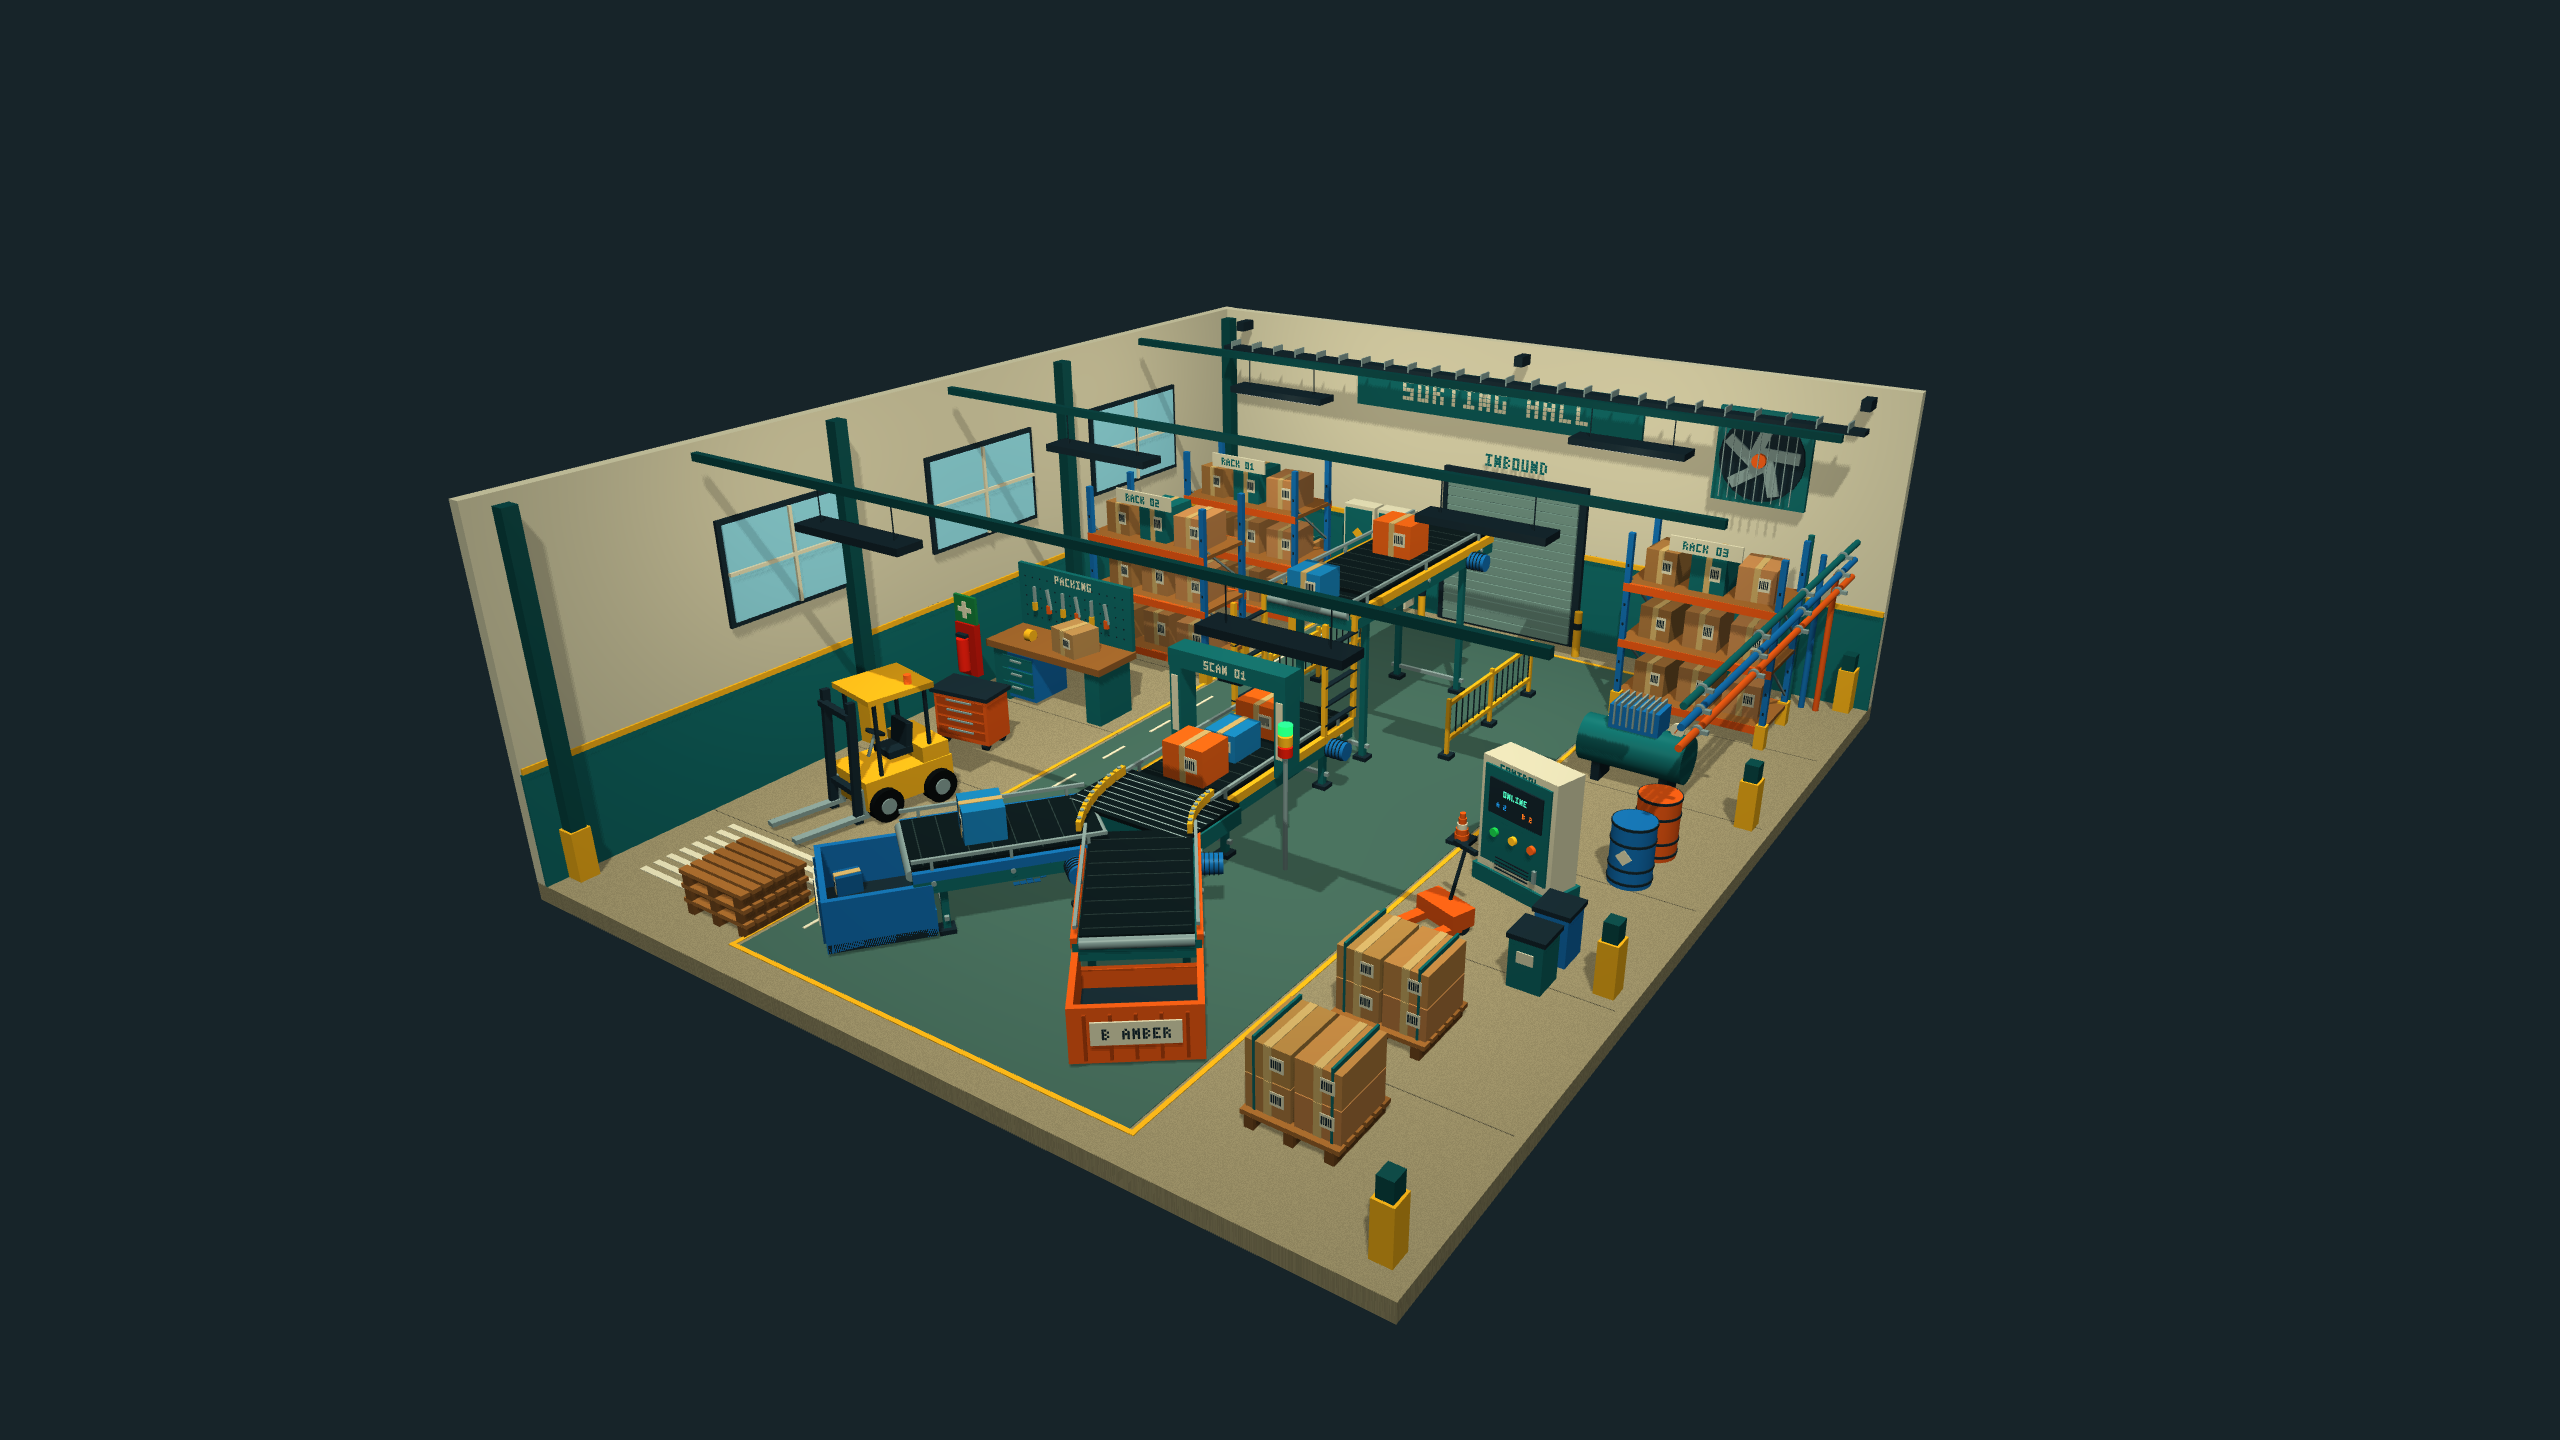
\includegraphics[width=0.74\textwidth]{assets/overview.png}\par
\vspace{6mm}
\begin{tabular}{rl}
\textbf{Student} & Rezuan Mustafa Hasan\\
\textbf{Roll} & 2107075\\
\textbf{Year} & 4th\\
\textbf{Semester} & 1st\\
\textbf{Course no} & CSE 4102\\
\textbf{Course title} & Computer Graphics and Image Processing\\
\textbf{Report date} & 7 October 2026
\end{tabular}
\vfill
\end{titlepage}
\setcounter{page}{2}
\section{System overview}
\label{sec:visual_tour}
The project simulates an automated warehouse sorting system using OpenGL. Boxes enter on an upper conveyor, fall onto a lower conveyor, stop for a simulated scan, and follow one of two exits. Blue boxes are directed to bin A, while orange boxes are directed to bin B.
\begin{shot}{assets/overview.png}{The complete rendered factory. Labels identify the sorting machine and the surrounding objects.}
\callout{0.47,0.56}{0.19,0.80}{Sorting machine}
\callout{0.35,0.48}{0.18,0.34}{Parked forklift}
\callout{0.67,0.59}{0.78,0.82}{Storage racks}
\callout{0.59,0.445}{0.83,0.30}{Control cabinet}
\callout{0.69,0.69}{0.87,0.66}{Wall fan}
\end{shot}
\subsection{Sorting sequence}
\begin{enumerate}
\item \textbf{Entry and transport:} colored cuboid parcels travel on the upper conveyor.
\item \textbf{Transfer and scanning:} a parcel falls onto the lower belt, then waits 0.65 s at the scanner.
\item \textbf{Routing and collection:} the gate aligns with the assigned route. The parcel turns, drops into its bin, and increments the corresponding counter.
\end{enumerate}
\note{The scanner is simulated, and the destination is assigned when a parcel is spawned. The gate and parcel trajectory use coordinated animations.}
\subsection{Technical specifications}
\par{\small\begin{tabularx}{\textwidth}{@{}L{34mm}Y@{}}\toprule
Software & C++17, OpenGL 3.3 Core requested, GLSL 330, CMake 3.20+.\\
Dependencies & GLFW 3.3.9, GLAD 2.0.6, GLM 0.9.9.8.\\
Scene construction & Reusable cubes and cylinders; no imported factory model or image texture.\\
Simulation and rendering & 12 reusable parcel slots, four point lights, daylight and shadows.\\\bottomrule
\end{tabularx}}\par

\clearpage
\section{Proposed and implemented features}
\label{sec:feature_comparison}
The proposed features are compared with the current C++ and GLSL implementation. \implemented{} indicates a completed feature; \adapted{} indicates a modification to the original design.
\par{\small\begin{tabularx}{\textwidth}{@{}L{38mm}L{27mm}Y@{}}\toprule
\textbf{Original proposal} & \textbf{Status} & \textbf{Final implementation}\\\midrule
Conveyor, rails, legs, exits & \implemented & Two height levels and two branch belts; scaled cube/cylinder assemblies (p.~\pageref{sec:machine_objects}).\\
Different moving boxes & \implemented & Four sizes, two colors and a fixed pool of 12 slots (p.~\pageref{sec:machine_objects}).\\
Rotating rollers & \implemented & Eight end rollers and moving belt strips; transfer-deck rollers remain static (p.~\pageref{sec:transfer}).\\
Flat gate at a pivot & \adapted & A rotating drive/linkage and articulated guide segments replace one flat board (pp.~\pageref{sec:scanner_gate}--\pageref{sec:routes}).\\
Green/red route lamp & \adapted & A red/yellow/green status tower shows pause/scan/run. Routes use blue/orange colors; the exact route lamp was not implemented (p.~\pageref{sec:controls}).\\
Floor plane & \implemented & Thin cuboid floor, work zone, safety lines and procedural grain (pp.~\pageref{sec:objects_modelling},\pageref{sec:lights}).\\
Model transformations & \implemented & Translation, rotation, scale and parent-child transforms (p.~\pageref{sec:objects_modelling}).\\
Box, roller, gate motion & \implemented & Time-based updates, gravity, animated angles and gate targets (pp.~\pageref{sec:transfer}--\pageref{sec:routes}).\\
Overhead point lighting & \implemented & Four warm lights, distance attenuation and a light toggle (p.~\pageref{sec:lights}).\\
Phong shading & \implemented & Per-fragment lighting with Blinn-Phong highlights; Gouraud mode added (p.~\pageref{sec:shading}).\\
Angled and top views & \implemented & Overview/top/side presets, free camera, mouse look and zoom (p.~\pageref{sec:controls}).\\
Pause, speed, gate keys & \implemented & Keyboard callbacks and held camera movement (p.~\pageref{sec:controls}).\\
Continuous operation & \implemented & Timed spawning, counting, collection and slot reuse (p.~\pageref{sec:routes}).\\\bottomrule
\end{tabularx}}\par
\subsection{Features added to the final project}
Two-level gravity transfer; scanner feedback; queue spacing; gate reservation; curved routes; labeled collection bins; counters; factory racks, vehicles and tools; rotating fan; directional shadows; Gouraud comparison; camera cutaway; reset; frame capture; simulation tests.

\subsection{Simulation architecture}
Each parcel stores its position, dimensions, destination and stage. \code{FactorySimulation} updates this data; \code{FactoryScene} renders it. Gate and parcel motion use prescribed trajectories rather than calculated contact forces. Queue rules maintain parcel spacing.

\clearpage
\section{Machine parts and specifications}
\label{sec:machine_objects}
\begin{shot}{assets/machine_detail.png}{Main machine at 24 s. The same blue/orange route colors continue from boxes to exits and bins.}
\callout{0.62,0.86}{0.79,0.91}{1 Upper belt}
\callout{0.46,0.65}{0.19,0.77}{2 Scanner}
\callout{0.39,0.49}{0.18,0.50}{3 Guide gate}
\callout{0.14,0.30}{0.16,0.14}{4 Blue bin A}
\callout{0.40,0.14}{0.77,0.08}{5 Orange bin B}
\callout{0.77,0.47}{0.83,0.61}{6 Cabinet}
\end{shot}
All lengths are expressed in scene units. The $x$ axis represents the lateral direction, the $y$ axis represents height, and the $z$ axis represents the longitudinal direction. Dimensions are given as width, height and length before rotation.
\par{\small\begin{tabularx}{\textwidth}{@{}L{34mm}Y@{}}\toprule
\textbf{Part} & \textbf{Specification}\\\midrule
Upper conveyor & Centre $(0,4.00,-4.50)$; width 2.10; length 6.70; end $z=-1.15$.\\
Lower conveyor & Centre $(0,1.45,1.48)$; width 2.10; length 5.36. Belt tops are 0.10 above base height.\\
Branch belts & Width 2.00; yaw $\pm37.5^\circ$; 1.80-unit turn plus 3.70-unit straight exit.\\
Scanner and gate & Scanner $z=1.75$; beam $(3.00,0.40,0.60)$ at $y=3.50$. Gate pivot $(0,1.45,4.00)$; seven guide pairs.\\
Collection bins & Base $(2.28,0.18,2.00)$; walls 1.10 high; floor top $y=0.30$; centers at route distance 6.15.\\
Rollers and cabinet & End roller diameter 0.23; legs $0.14\times0.14$. Cabinet body $(1.90,2.80,0.78)$, yaw $-16^\circ$.\\\bottomrule
\end{tabularx}}\par
\textbf{Four parcel sizes:} $(0.86,0.70,0.82)$, $(1.03,0.82,0.90)$, $(0.78,0.62,0.96)$, $(1.10,0.76,0.84)$. Bodies, tape, labels and five barcode-like strips share a parent transform.
\source{\code{include/FactorySimulation.h}: \code{FactoryLayout}; \code{src/FactoryScene.cpp}: conveyor, parcel, scanner, gate and bin drawing.}

\clearpage
\section{Conveyor movement and falling}
\label{sec:transfer}
\begin{figure}[H]\centering
\begin{minipage}{0.49\linewidth}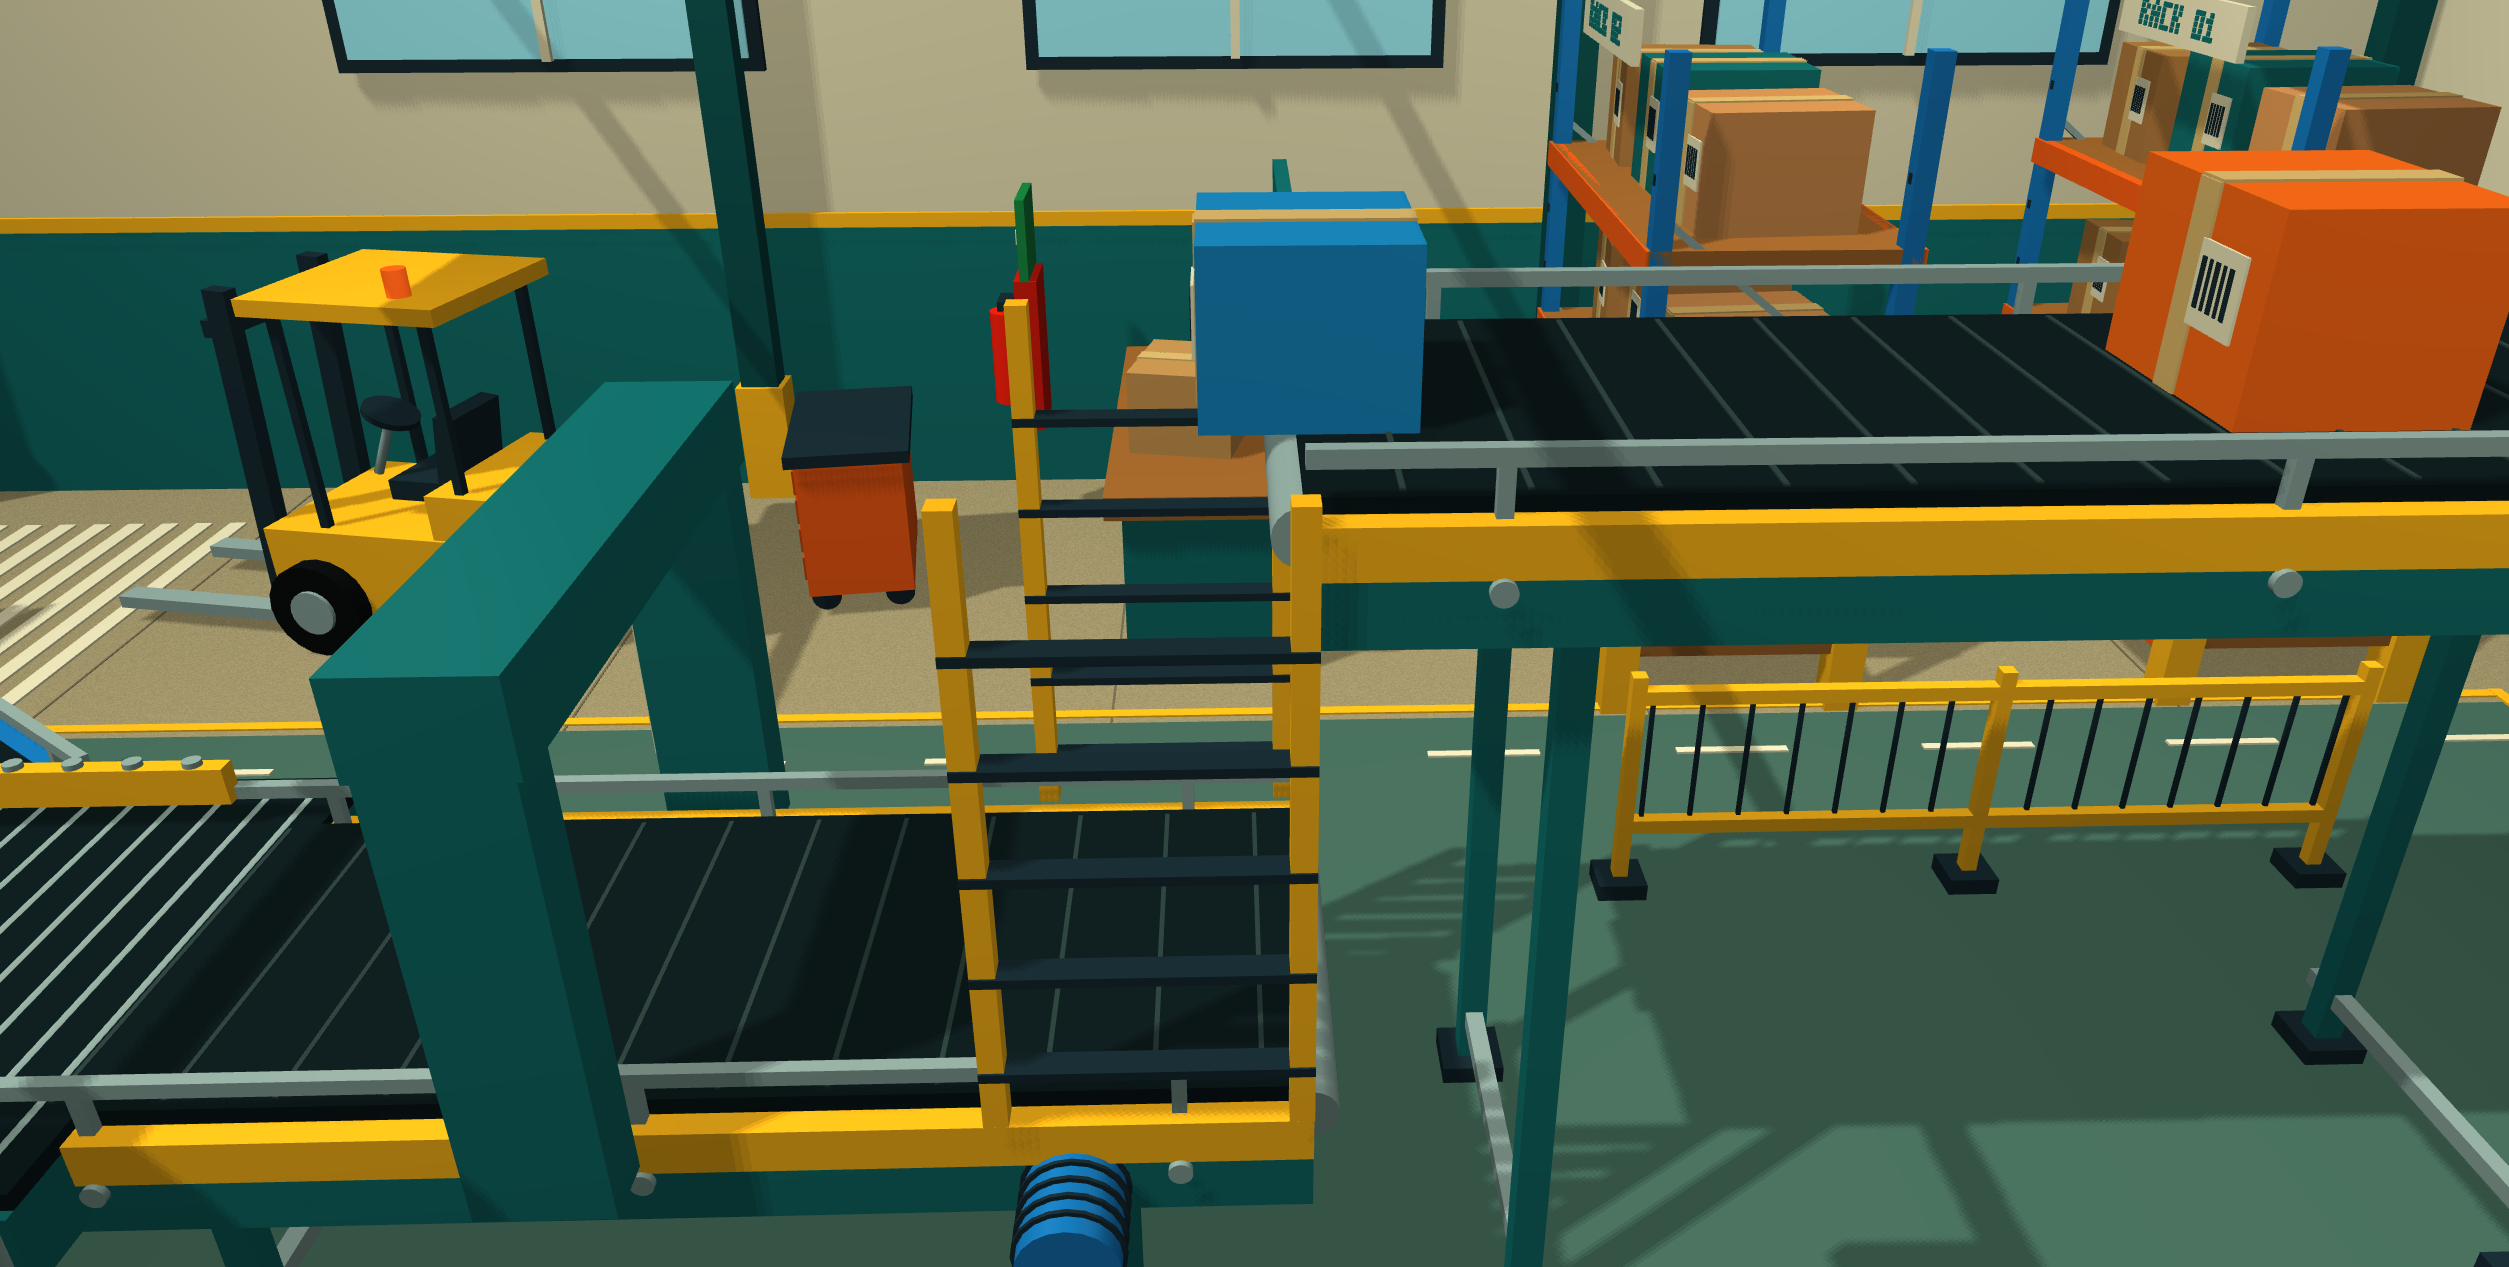
\includegraphics[width=\linewidth]{assets/transfer_before_crop.png}\par\small\textbf{A. 4.10 s:} first blue box approaches the upper belt edge.\end{minipage}\hfill
\begin{minipage}{0.49\linewidth}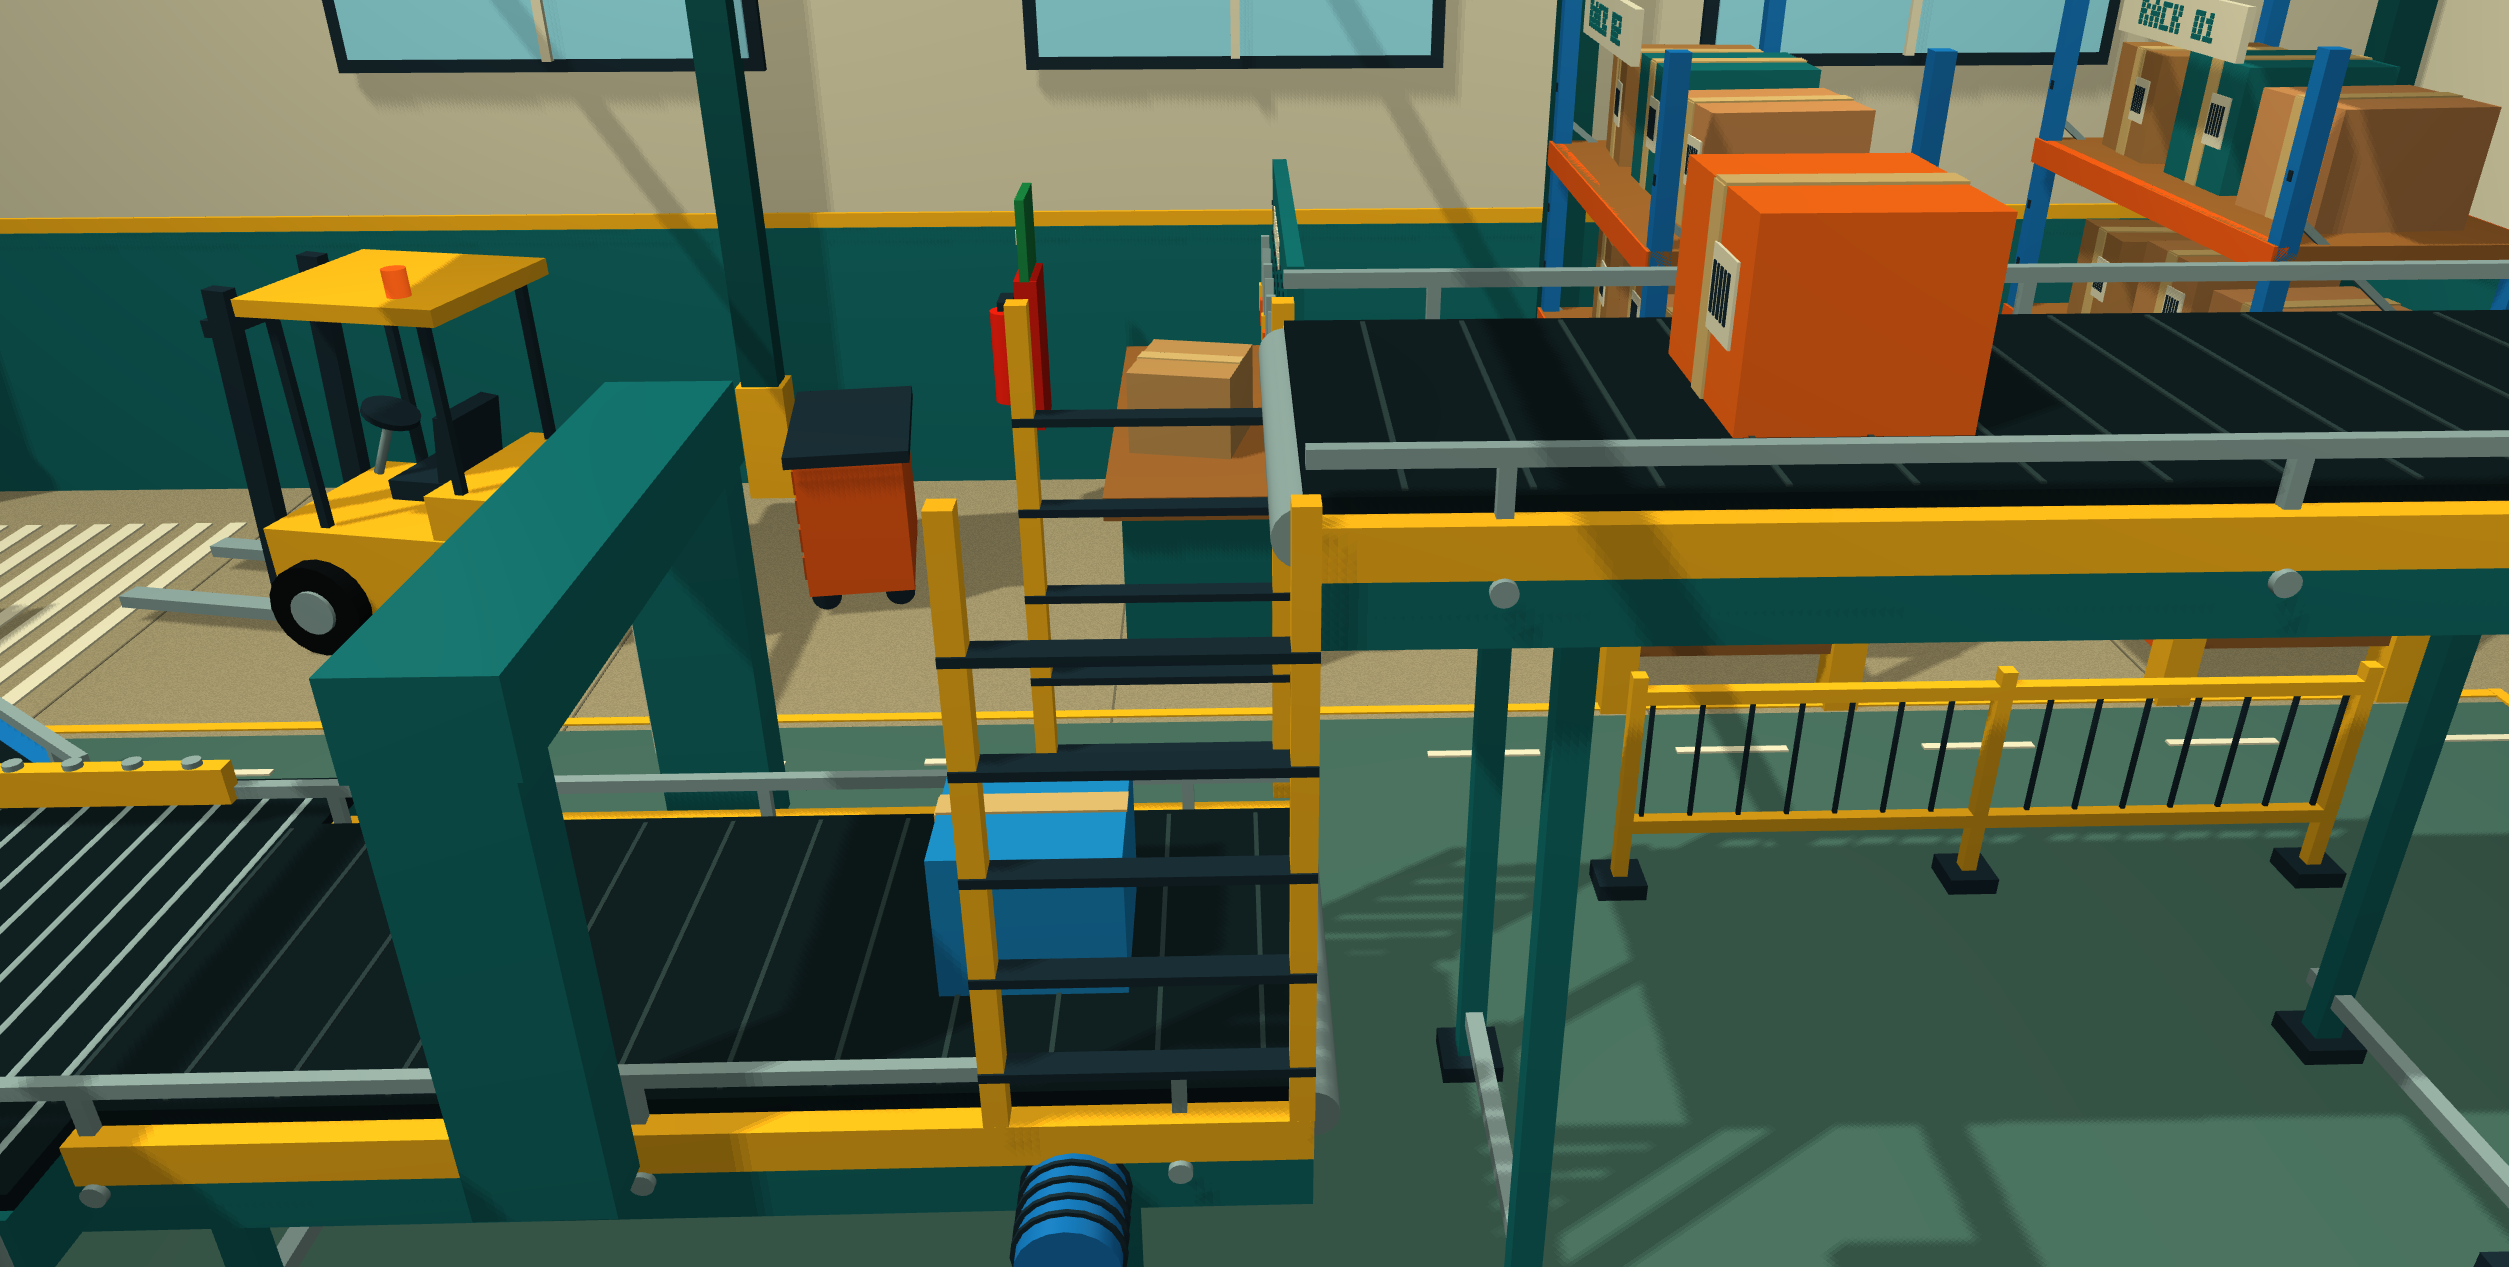
\includegraphics[width=\linewidth]{assets/transfer_landed_crop.png}\par\small\textbf{B. 5.30 s:} it has landed on the lower belt.\end{minipage}
\caption{Before and after the transfer, using the same camera and image crop.}
\end{figure}
\begin{shot}[0.80\linewidth]{assets/transfer_fall_crop.png}{At 4.75 s the box is falling and tilted. This close view shows the gap between the two conveyor levels.}
\callout{0.44,0.63}{0.20,0.90}{Falling box}
\callout{0.64,0.67}{0.85,0.94}{Upper belt}
\callout{0.22,0.15}{0.19,0.08}{Lower belt}
\end{shot}
\subsection{Motion model}
On a conveyor, the position update is $z'=z+v\Delta t$, where $v$ is speed and $\Delta t$ is elapsed time. The default speed is 1.55 units/s; keyboard input changes it by 0.20 within 0.65--3.00 units/s.

During a fall, the code first updates vertical velocity, then height:
\begin{equation}
v_y'=v_y-9.81\Delta t,\qquad y'=y+v_y'\Delta t.
\end{equation}
The parcel also moves forward by $0.62\Delta t$. On landing, the center height is constrained to $1.45+0.10+h/2$, where $h$ is box height. Tilt is $16^\circ\sin(\pi\min(1,t/0.72))$; it returns to zero on landing.

\textbf{Spacing:} required center gap is $(l_i+l_a)/2+0.40$. A box waits when the receiver is occupied. Updates use steps of at most $1/120$ s and cap a frame's accepted time at 0.25 s. End rollers use $\theta'= (\theta+190v\Delta t)\bmod360$; repeating strips suggest belt movement. These roller rates are visual choices.
\source{\code{FactorySimulation.cpp}: \code{update()}, \code{advanceOnBelt()}, falling case; \code{FactoryScene.cpp}: conveyor/box drawing.}

\clearpage
\section{Scanner and gate control}
\label{sec:scanner_gate}
\begin{shot}{assets/scanner_crop.png}{At 6.70 s the first blue parcel is in the Scanning state. The scanner frame, parcel label and scan line can be inspected at a larger scale.}
\callout{0.48,0.35}{0.21,0.15}{Stopped parcel}
\callout{0.47,0.51}{0.77,0.58}{Scan line}
\callout{0.46,0.84}{0.23,0.91}{Scanner frame}
\end{shot}
\subsection{Scanning and gate reservation}
\begin{enumerate}
\item At $z=1.75$, the parcel stops for \textbf{0.65 s}. A bright line sweeps across its top: $z_{line}=1.75+0.43l\sin(15t)$.
\item The parcel is marked scanned. Even spawn numbers correspond to the left/blue route; odd numbers correspond to the right/orange route. This assignment is made at spawning.
\item The most advanced scanning/approaching parcel reserves the gate. Other boxes wait while that owner passes.
\end{enumerate}
\subsection{Gate movement and release}
Left target is $-37.5^\circ$ and right target is $+37.5^\circ$. The code changes its angle by at most $85^\circ$/s:
\begin{equation}
\theta'=\theta+\operatorname{clamp}(\theta_{target}-\theta,-85\Delta t,85\Delta t).
\end{equation}
\code{clamp} limits a value to the given interval. A box enters only when it owns the gate and angle error is below $0.10^\circ$. Otherwise it waits at $z=4.00-l/2-0.42$. Ownership ends after route distance 2.75, or when the owner leaves the exit stage.

The gate contains a fixed pivot, rotating linkage and seven guide pairs, at $d_i=0.25+0.29i$ for $i=0,\ldots,6$. For current angle $\alpha$ in radians, each guide uses $\beta_i=\alpha\min(d_i/1.80,1)$ and radius $1.80/\alpha$. Side offsets are $\pm1.07$, producing the curved channel shown next. A straight case avoids division by zero near angle zero.
\note{\textbf{Manual gate control:} \code{G} alternates a requested angle for 2.25 s. Automatic ownership has priority; an occupied route remains stable.}
\source{\code{FactorySimulation.cpp}: scanning/approach cases, \code{step()}, \code{testGate()}; \code{FactoryScene.cpp}: \code{drawScannerAndGate()}.}

\clearpage
\section{Two exits and continuous operation}
\label{sec:routes}
\begin{figure}[H]\centering
\begin{minipage}{0.49\linewidth}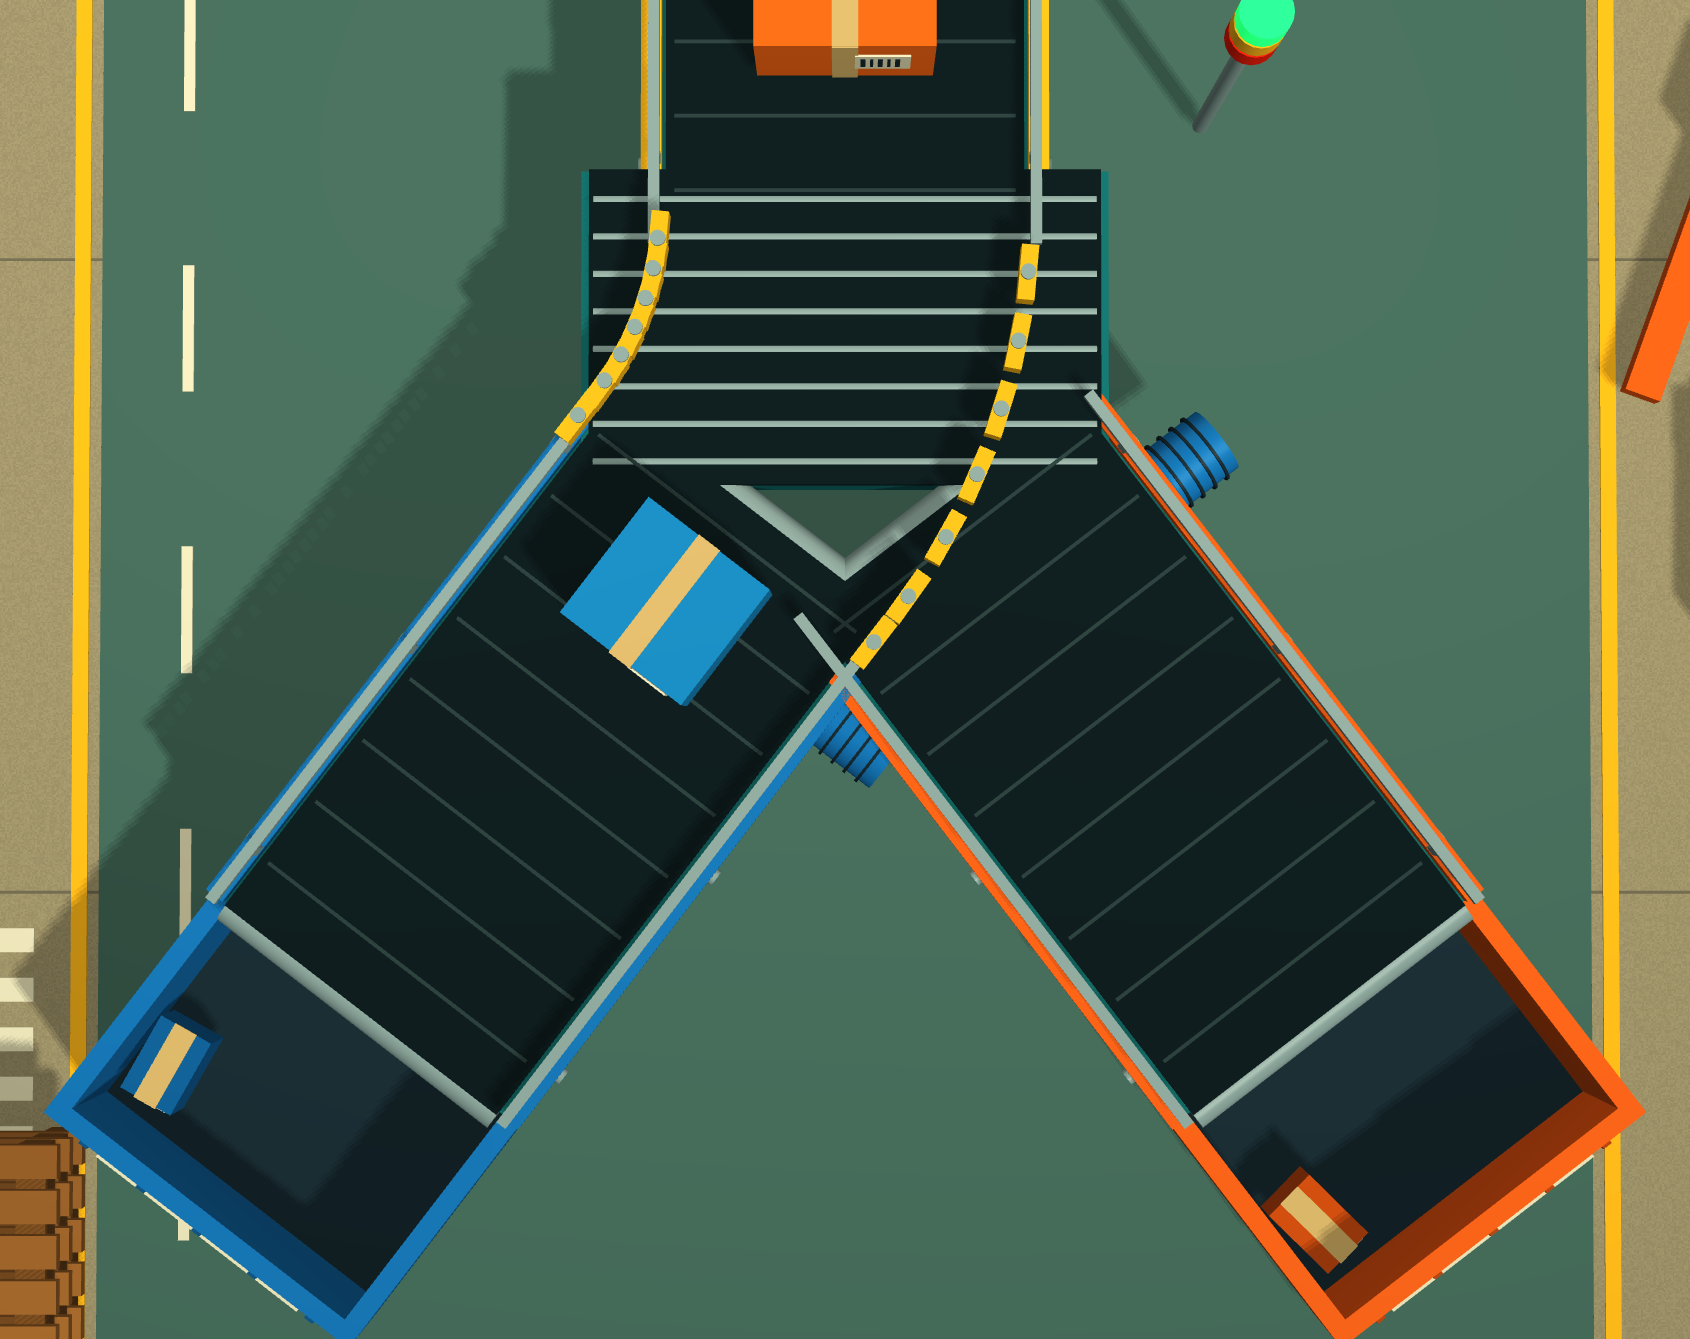
\includegraphics[width=\linewidth]{assets/gate_left_crop.png}\par\small\textbf{A. 10.20 s:} blue parcel on the left route; gate $-37.5^\circ$.\end{minipage}\hfill
\begin{minipage}{0.49\linewidth}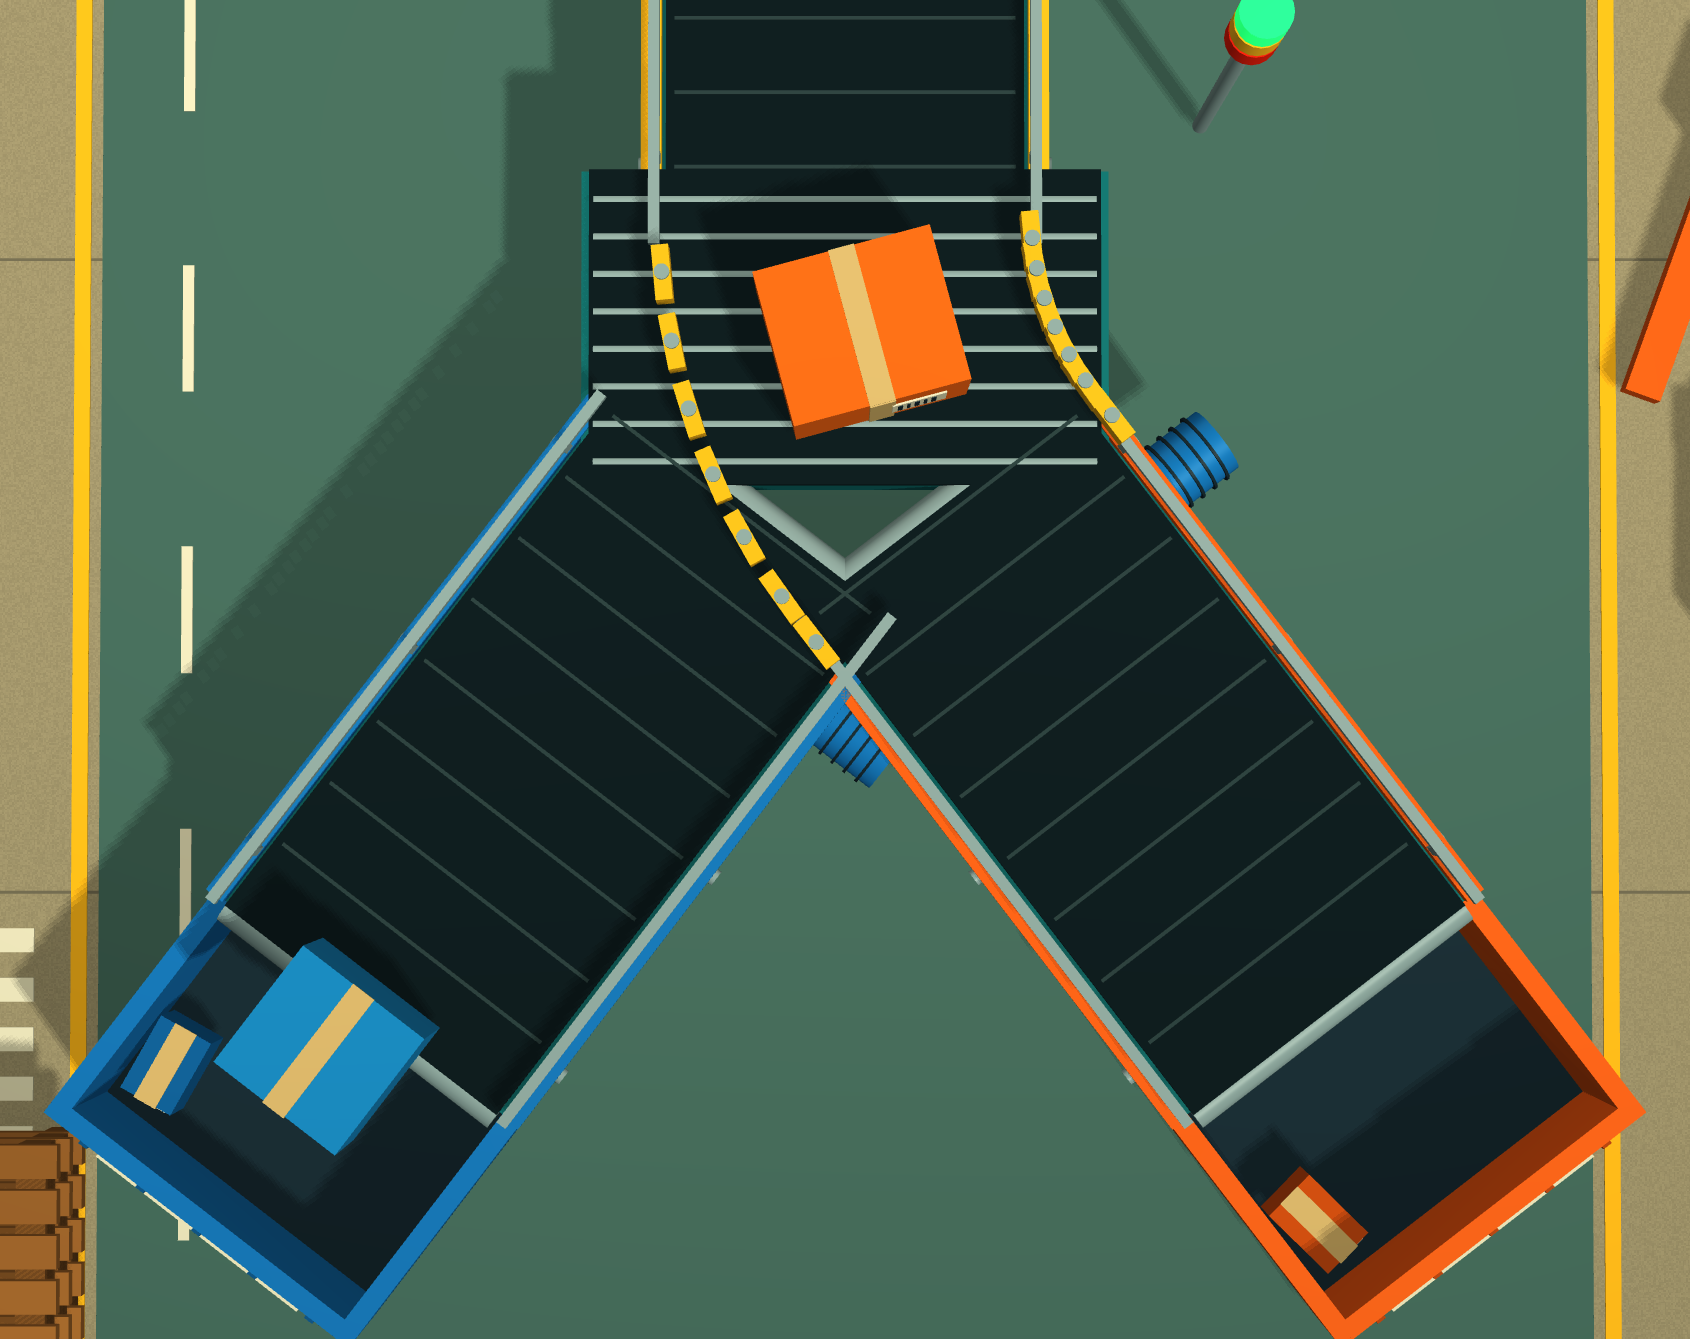
\includegraphics[width=\linewidth]{assets/gate_right_crop.png}\par\small\textbf{B. 12.25 s:} orange parcel starts the right route; gate $+37.5^\circ$.\end{minipage}
\caption{Matched overhead close-ups show the guide channel changing direction. Left and right refer to the machine's $x$ axis.}
\end{figure}
\subsection{Curved route model}
The first 1.80 units follow a circle, then the parcel follows a straight branch. Let $a=37.5^\circ$ in radians, $r=1.80/a\approx2.7502$, $s$ be route distance, $\sigma=-1$ for left or $+1$ for right, and $\beta=\operatorname{clamp}(s,0,1.80)/r$:
\begin{equation}
x=\sigma r(1-\cos\beta),\qquad z=r\sin\beta.
\end{equation}
These offsets start from $(0,1.55,4.00)$. After the arc, add $(\sigma\sin a,0,\cos a)\max(0,s-1.80)$. Center height is $1.55+h/2$. Yaw turns gradually as $\sigma37.5^\circ\operatorname{clamp}(s/1.80,0,1)$.
\begin{center}\begin{minipage}{0.67\linewidth}
\begin{shot}{assets/collection_crop.png}{At 13.15 s the first blue parcel has landed inside bin A. The recorded simulation state confirms Collected and counter A = 1.}
\callout{0.28,0.57}{0.19,0.81}{Collected blue box}
\callout{0.68,0.70}{0.80,0.88}{Exit belt}
\end{shot}
\end{minipage}\end{center}
\textbf{Collection and reuse:} the rear must clear the 5.50-unit route before dropping. Gravity lowers the box to $y=0.30+h/2$; its counter increases once. After 0.65 s the slot becomes free. A new parcel can spawn every 2.50 s when a slot and entry space are available. The 12-slot pool keeps the factory running without unlimited accumulation. One small static cargo box remains in each bin as decoration.
\source{\code{FactorySimulation.cpp}: \code{routePosition()}, \code{routeYaw()}, exit/drop/collection cases, \code{spawnBox()}.}

\clearpage
\section{Geometric modelling and transformations}
\label{sec:objects_modelling}
\begin{figure}[H]\centering
\begin{minipage}{0.49\linewidth}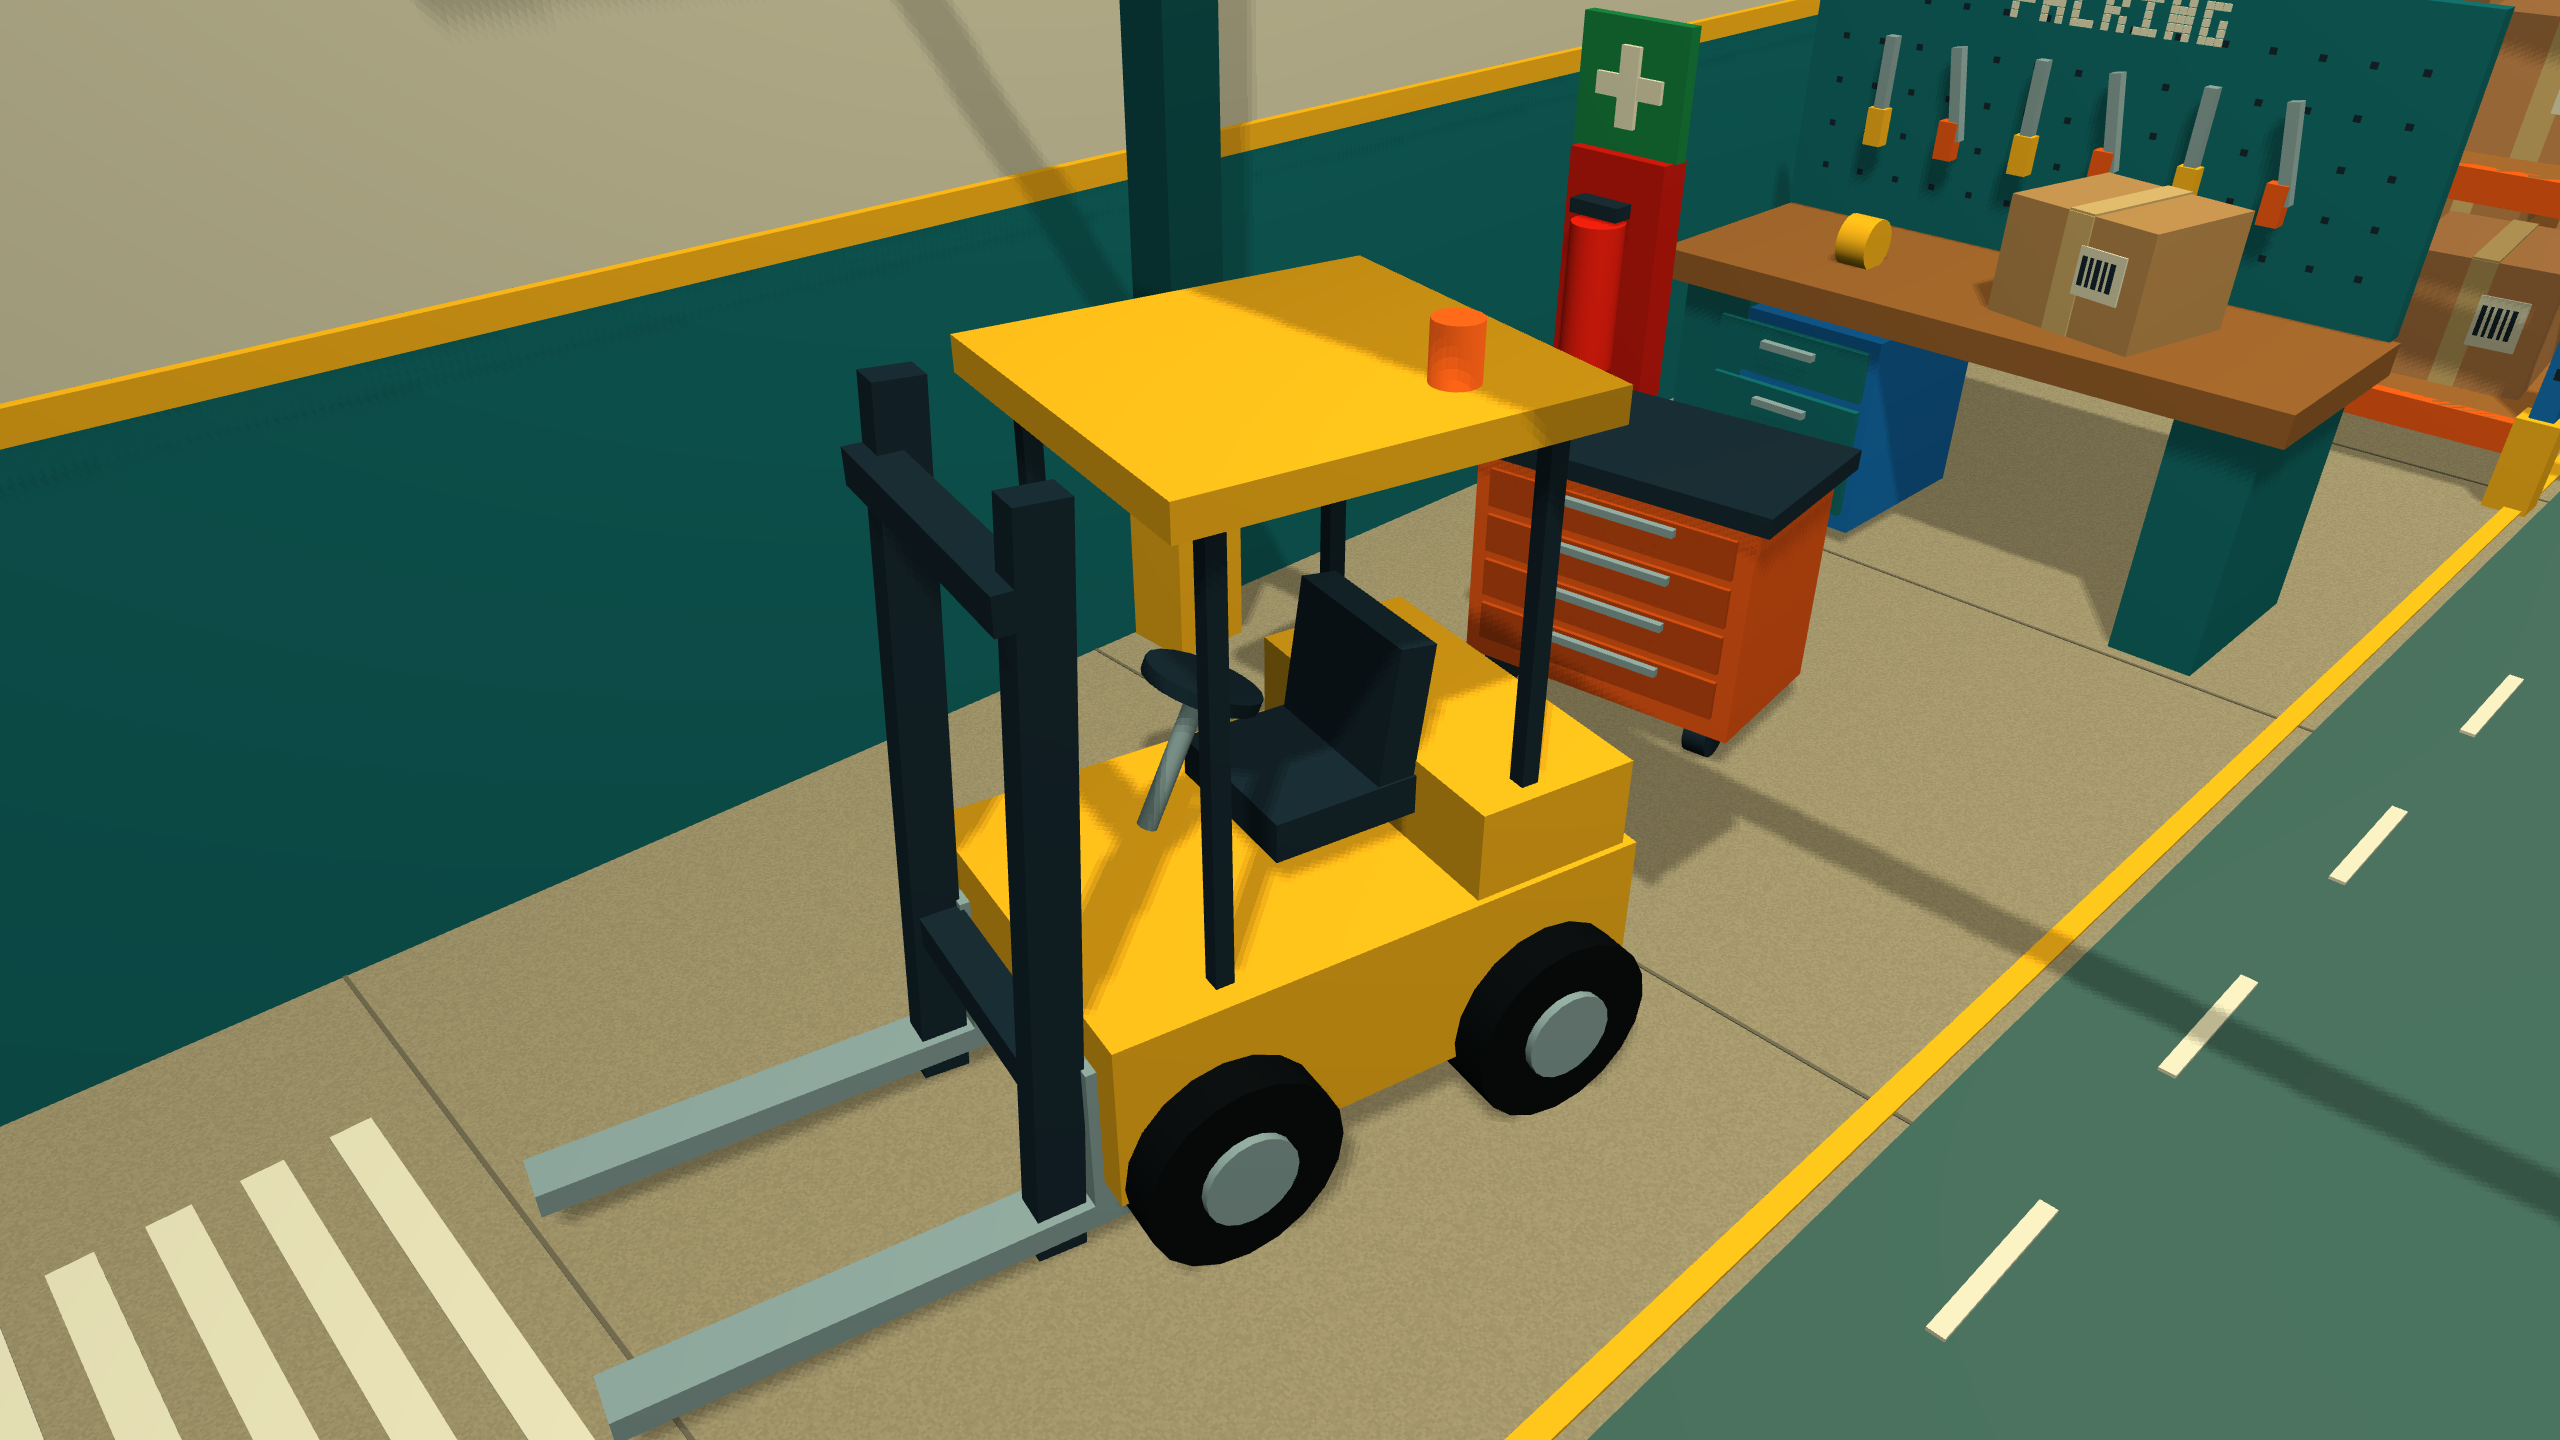
\includegraphics[width=\linewidth]{assets/forklift_crop.png}\par\small\textbf{Forklift:} cube body/forks and cylinder wheels.\end{minipage}\hfill
\begin{minipage}{0.49\linewidth}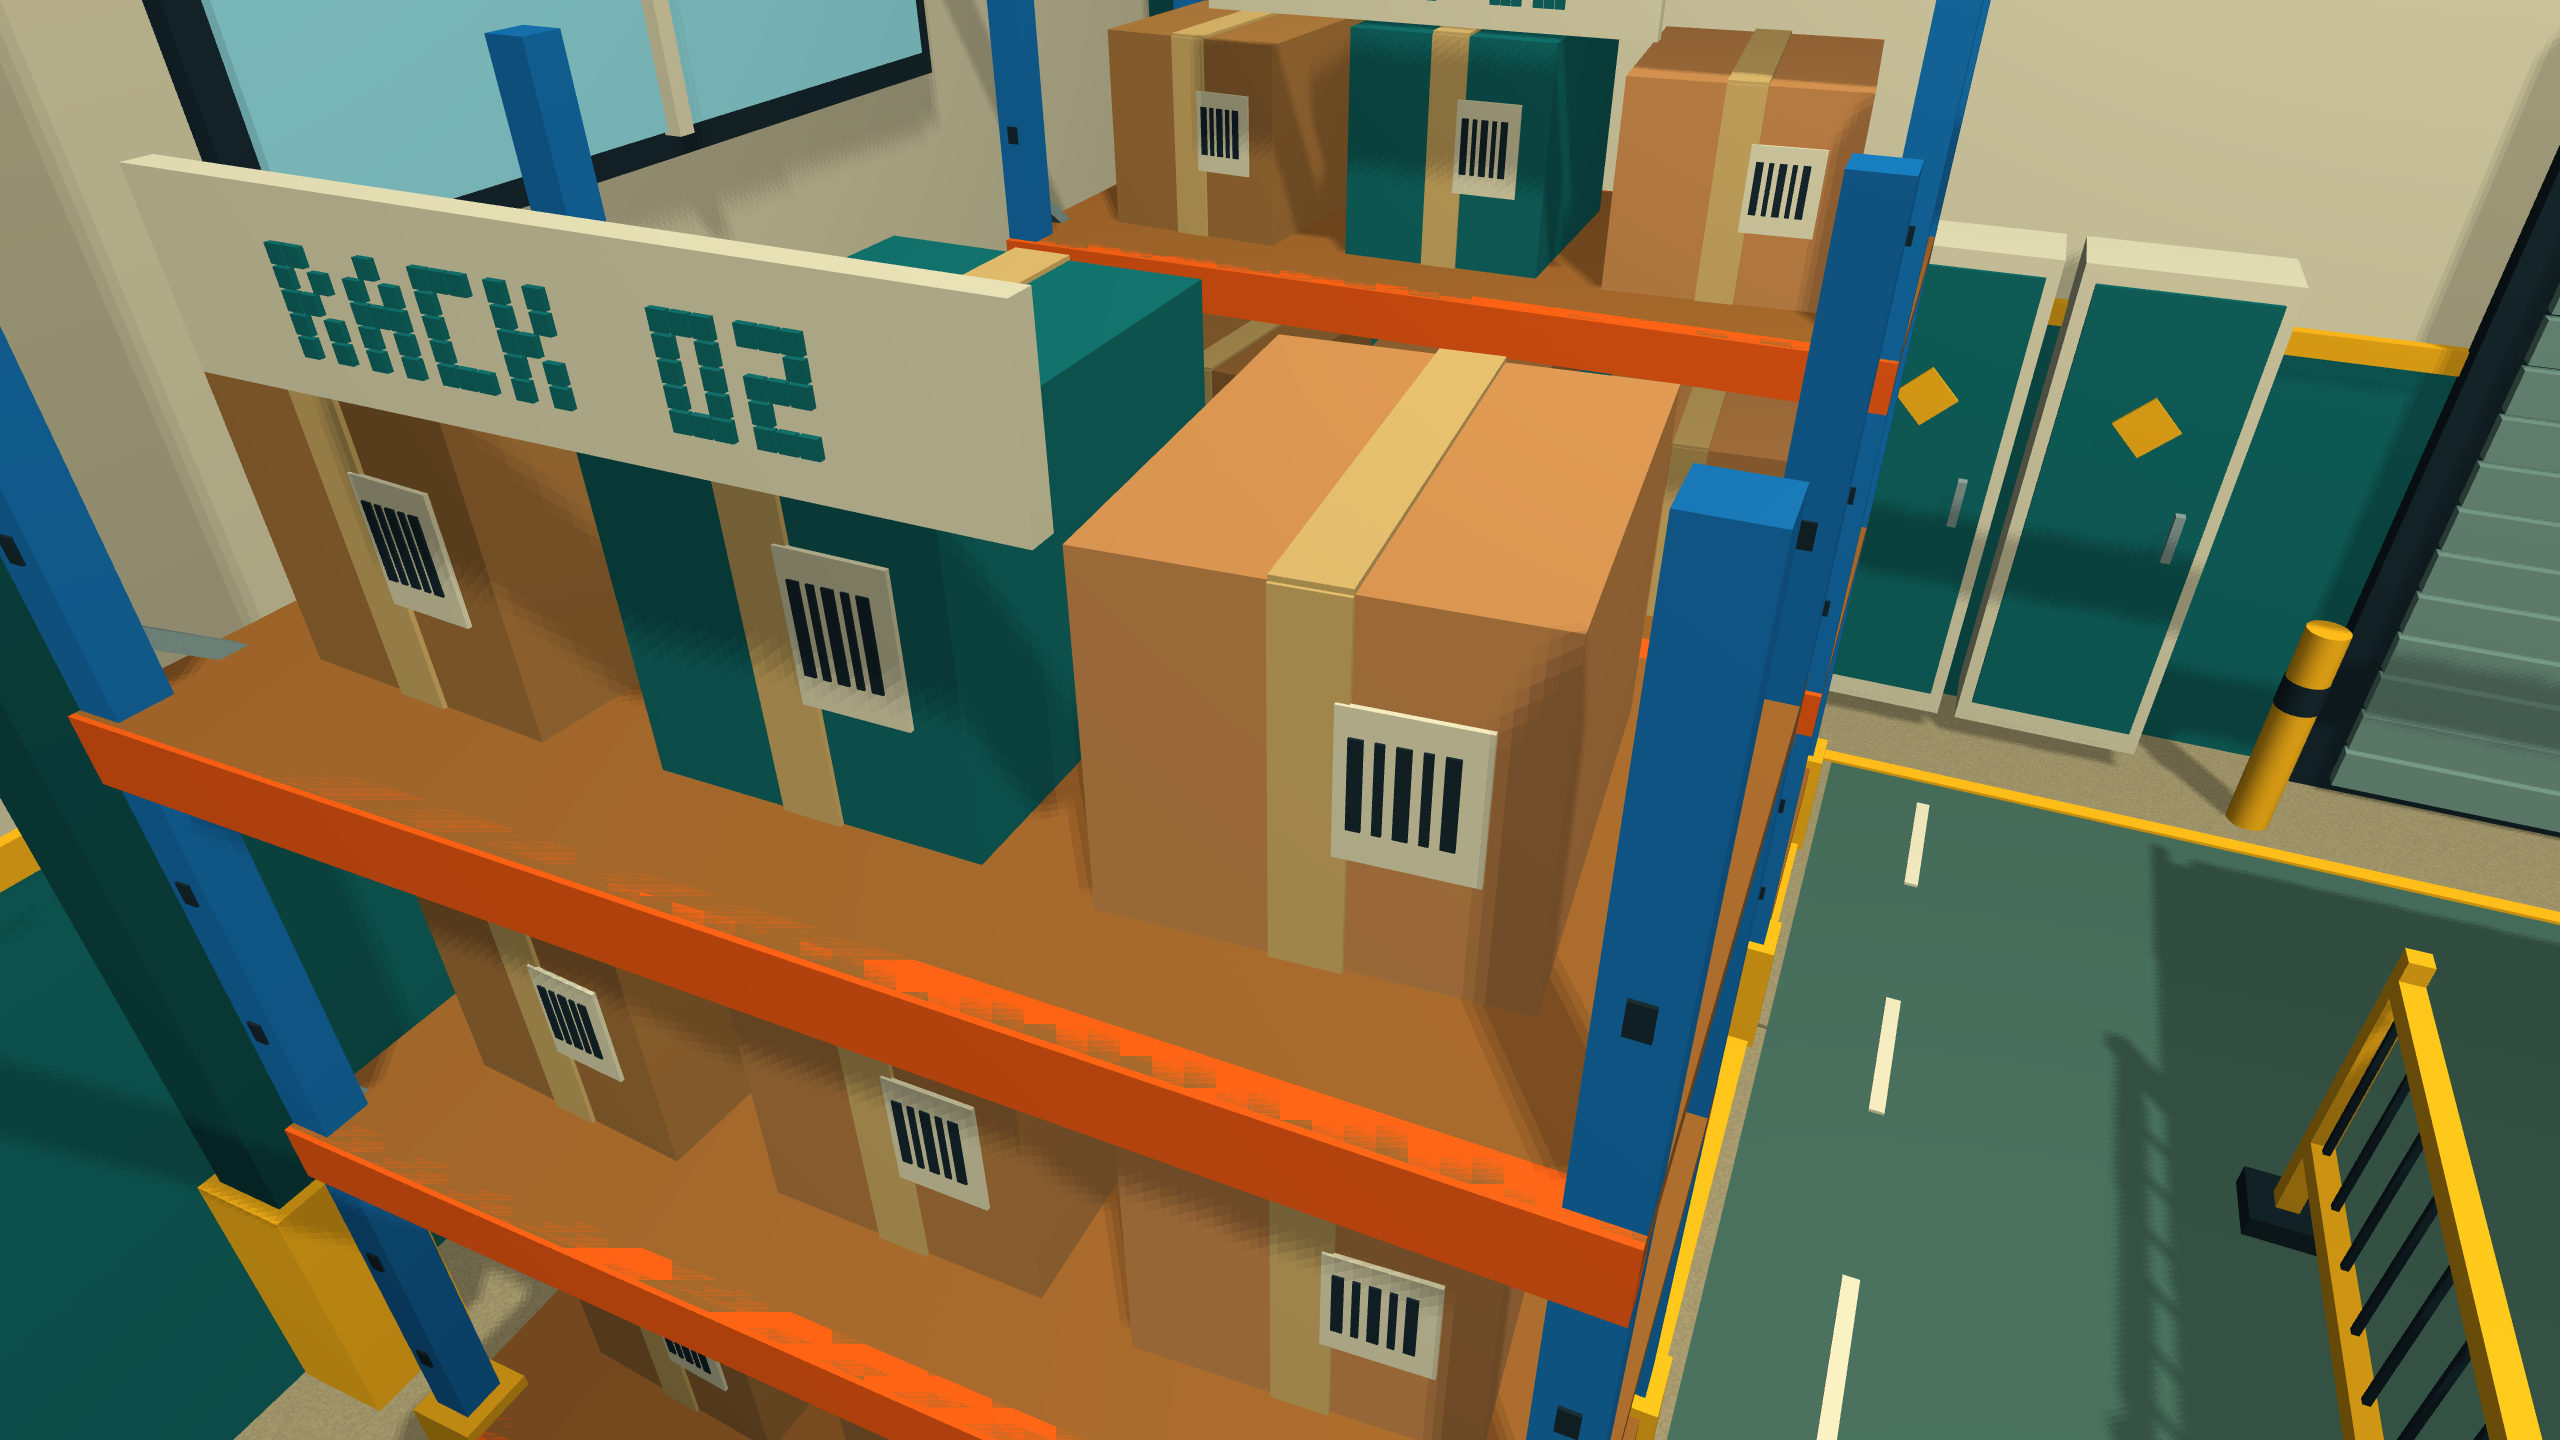
\includegraphics[width=\linewidth]{assets/racks_crop.png}\par\small\textbf{Racks:} repeated posts, shelves and parcels.\end{minipage}
\vspace{3mm}
\begin{minipage}{0.49\linewidth}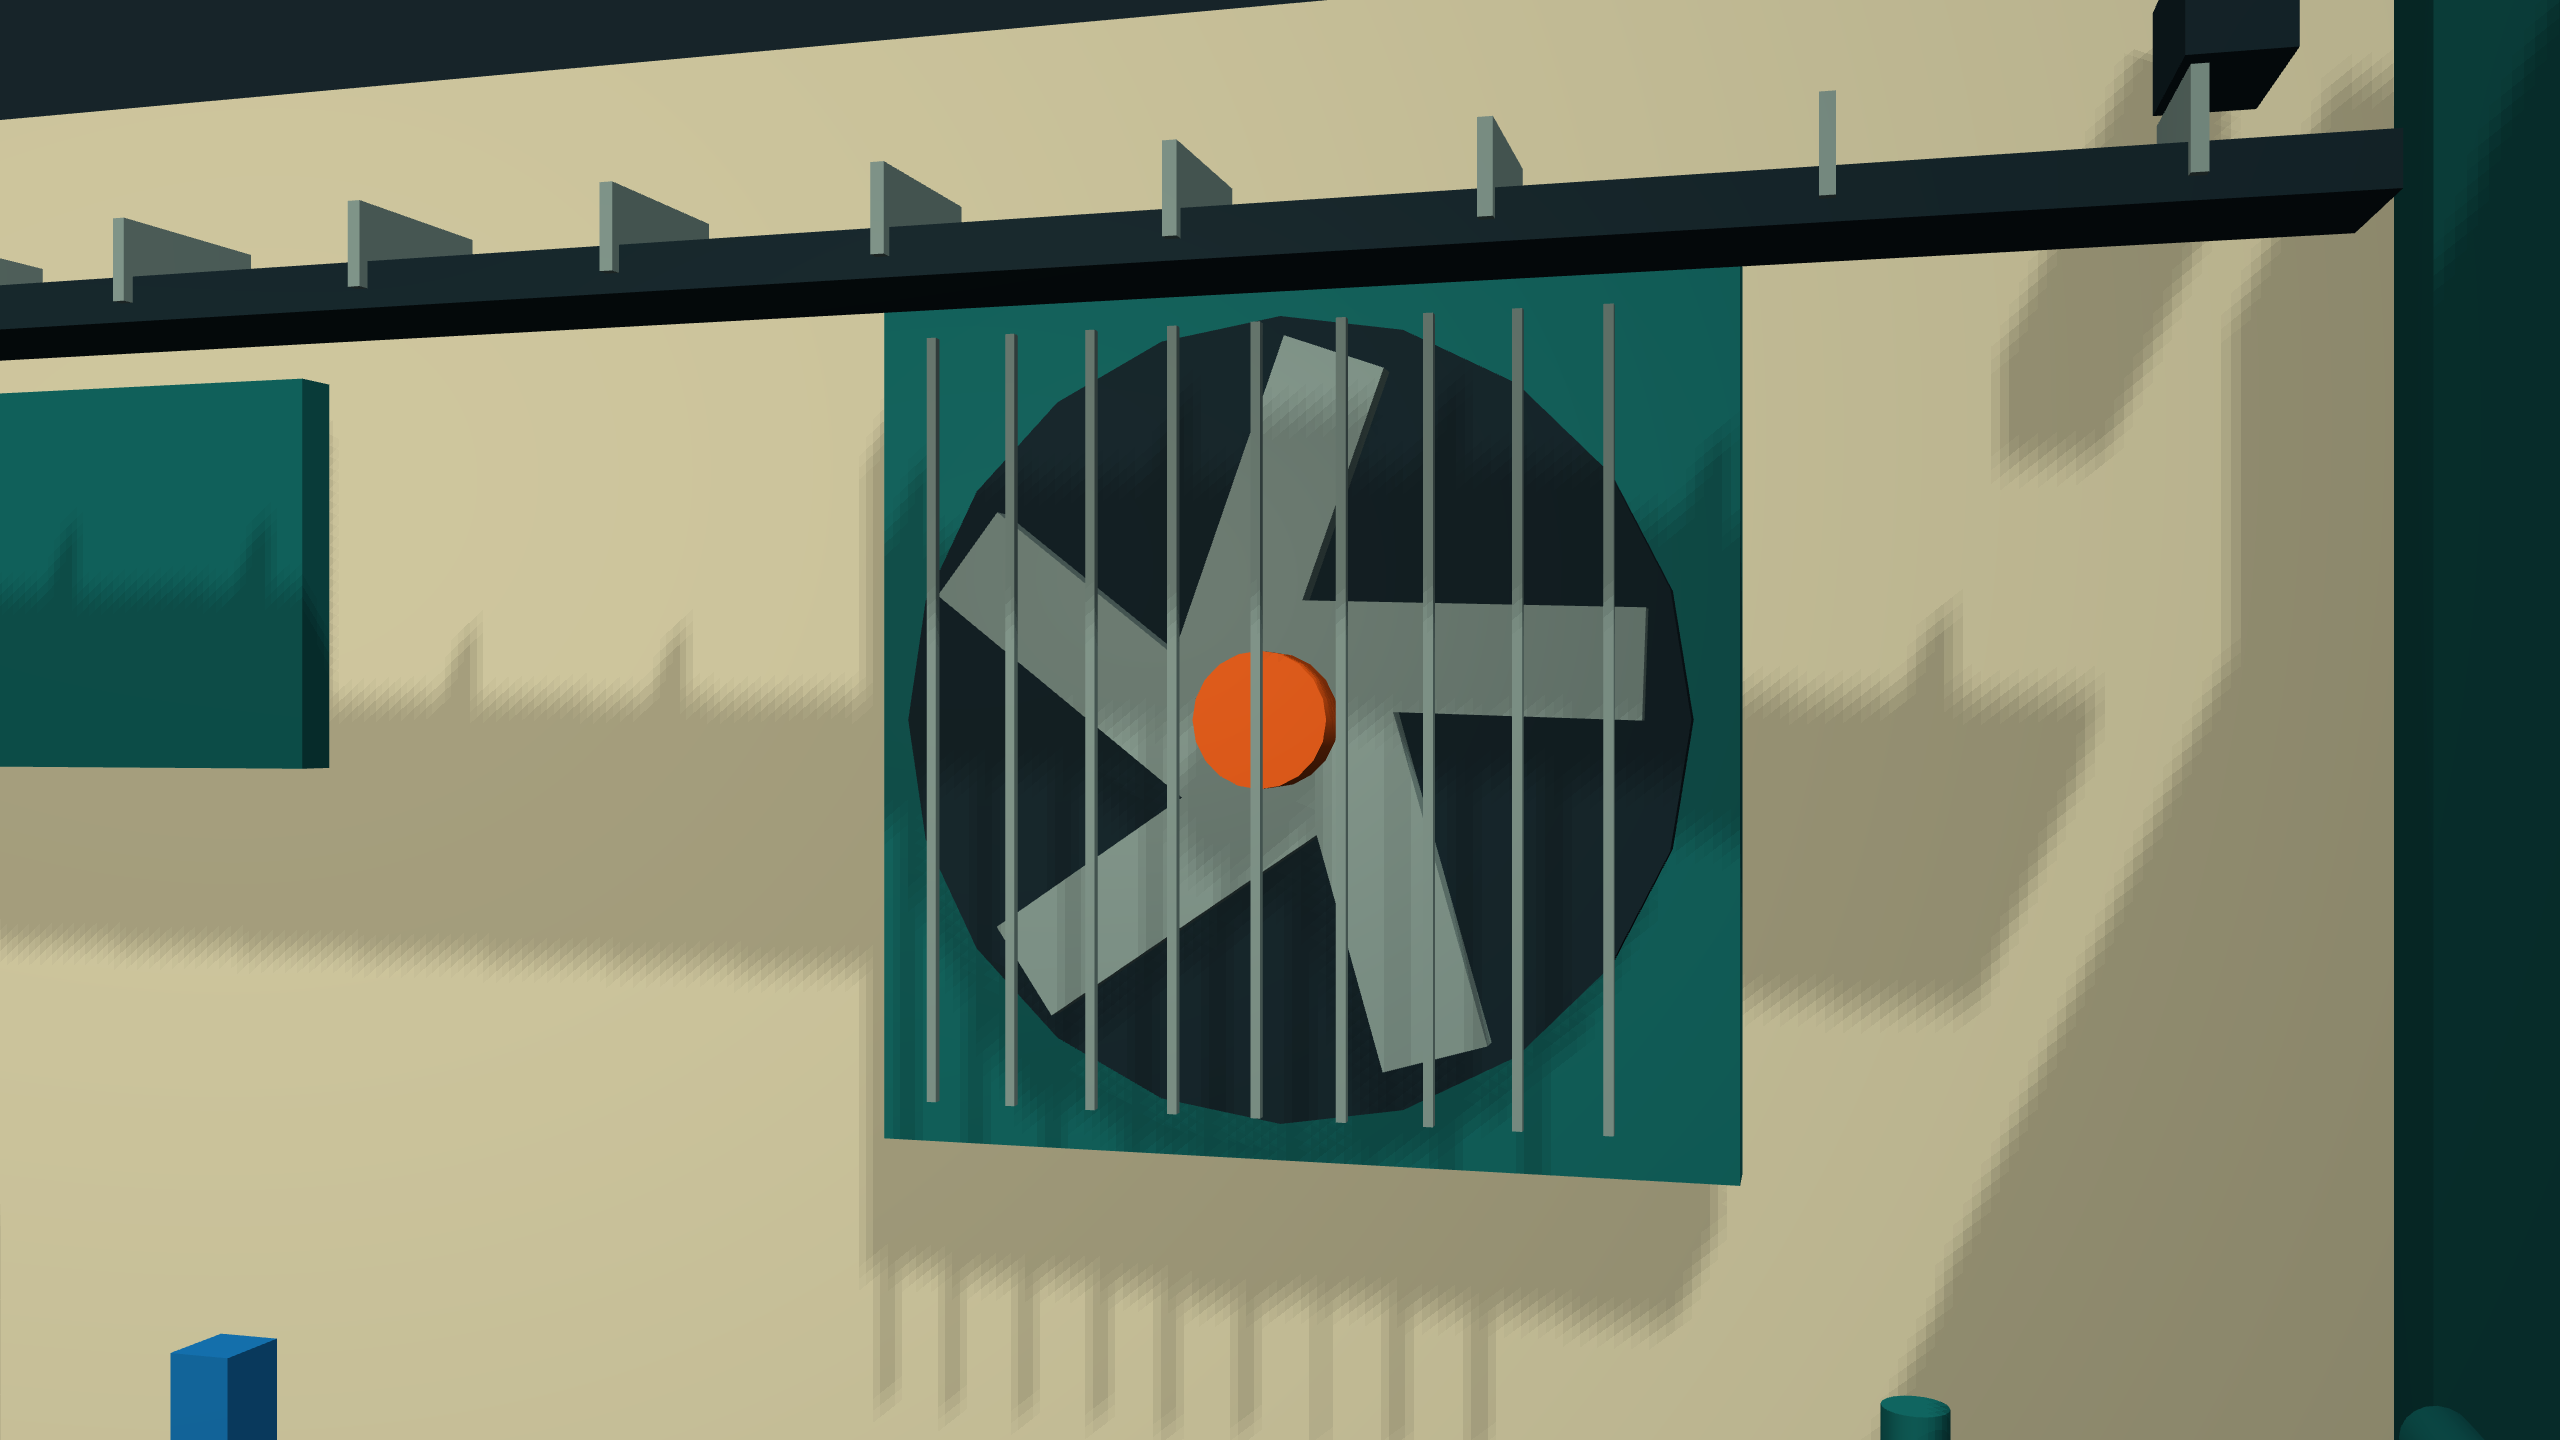
\includegraphics[width=\linewidth]{assets/fan_crop.png}\par\small\textbf{Fan:} five blades rotate around one hub.\end{minipage}\hfill
\begin{minipage}{0.49\linewidth}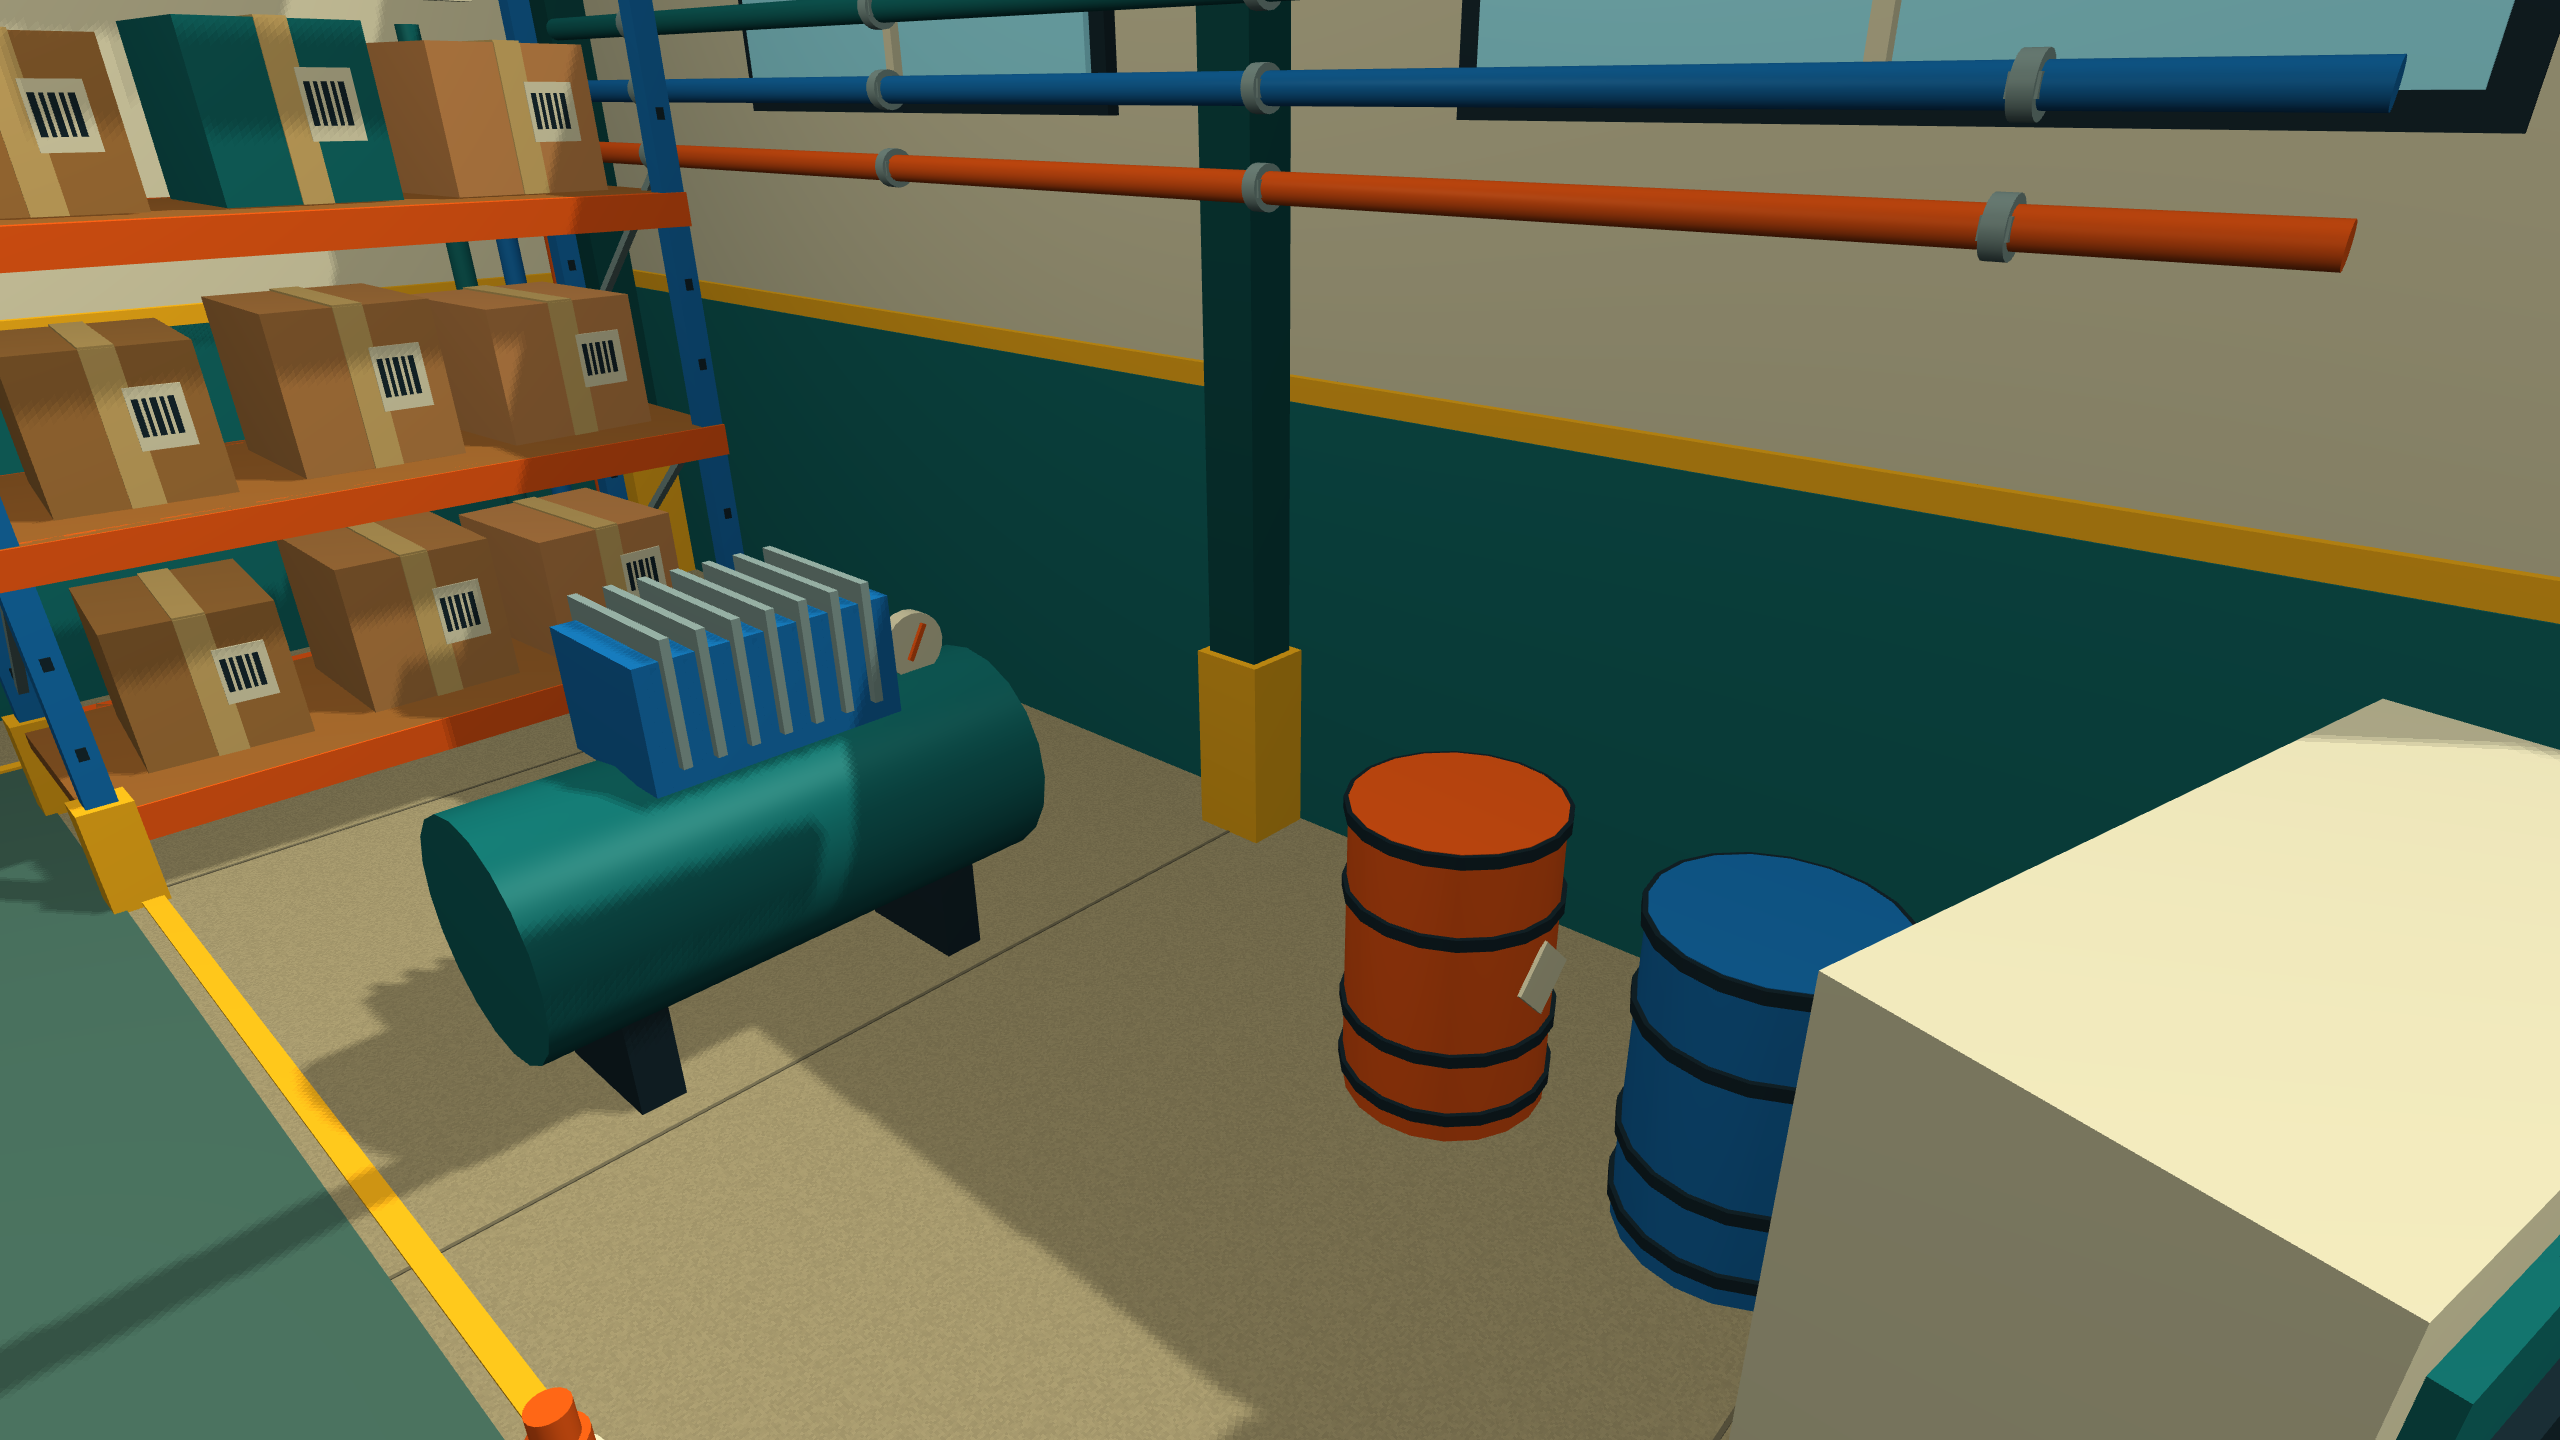
\includegraphics[width=\linewidth]{assets/utilities_crop.png}\par\small\textbf{Utilities:} cylinders form tanks, drums and pipes.\end{minipage}
\caption{Actual close-ups of environment objects. The forklift and utility objects are static; the fan is animated.}
\end{figure}
\subsection{Primitive geometry and hierarchical transforms}
A unit cube has 12 triangles and 36 vertex entries. Scaling it makes belts, legs, shelves and boxes. A 20-segment cylinder has 86 vertex entries and 80 triangles; circular vertices use $x=0.5\cos\theta$, $z=0.5\sin\theta$, $\theta=2\pi i/20$.

The shared helper builds $M=T R_y R_x R_z S$: scale the local shape, rotate it, then place it. Attached parts use $M_{part}=M_{parent}M_{local}$. This keeps labels on boxes and blades around the fan hub. The fan uses $\theta_f'=(\theta_f+150\Delta t)\bmod360$ and keeps turning while sorting is paused.
\par{\small\begin{tabularx}{\textwidth}{@{}L{34mm}Y@{}}\toprule
\textbf{Object} & \textbf{Selected specifications}\\\midrule
Room and floor & $20\times8\times24$ room; floor $(20,0.40,24)$; open front, no solid roof.\\
Racks and loads & Three racks, three shelves each, three cartons per shelf: 27 rack cartons. Three staged pallet loads hold four cartons each.\\
Fan and vehicles & Fan housing diameter 2.12; forklift tyre diameter 0.76; pallet-truck forks length 1.90.\\
Utilities and lettering & Drum diameter 0.90, height 1.38; tank diameter 1.10, length 2.45. Text uses a $3\times5$ cuboid-cell stencil.\\\bottomrule
\end{tabularx}}\par
Normals use $\mathbf{N}=\operatorname{normalize}((M_{3\times3}^{-1})^T\mathbf{n})$, preserving their orientation after non-uniform scaling. The final vertex position is $PVM\mathbf{p}$, using projection, view and model matrices.
\source{\code{Geometry.cpp}: cube/cylinder meshes; \code{FactoryScene.cpp}: transforms, text, environment and fan drawing.}

\clearpage
\section{Lighting and shading in the scene}
\label{sec:shading}
\begin{figure}[H]\centering
\begin{minipage}{0.49\linewidth}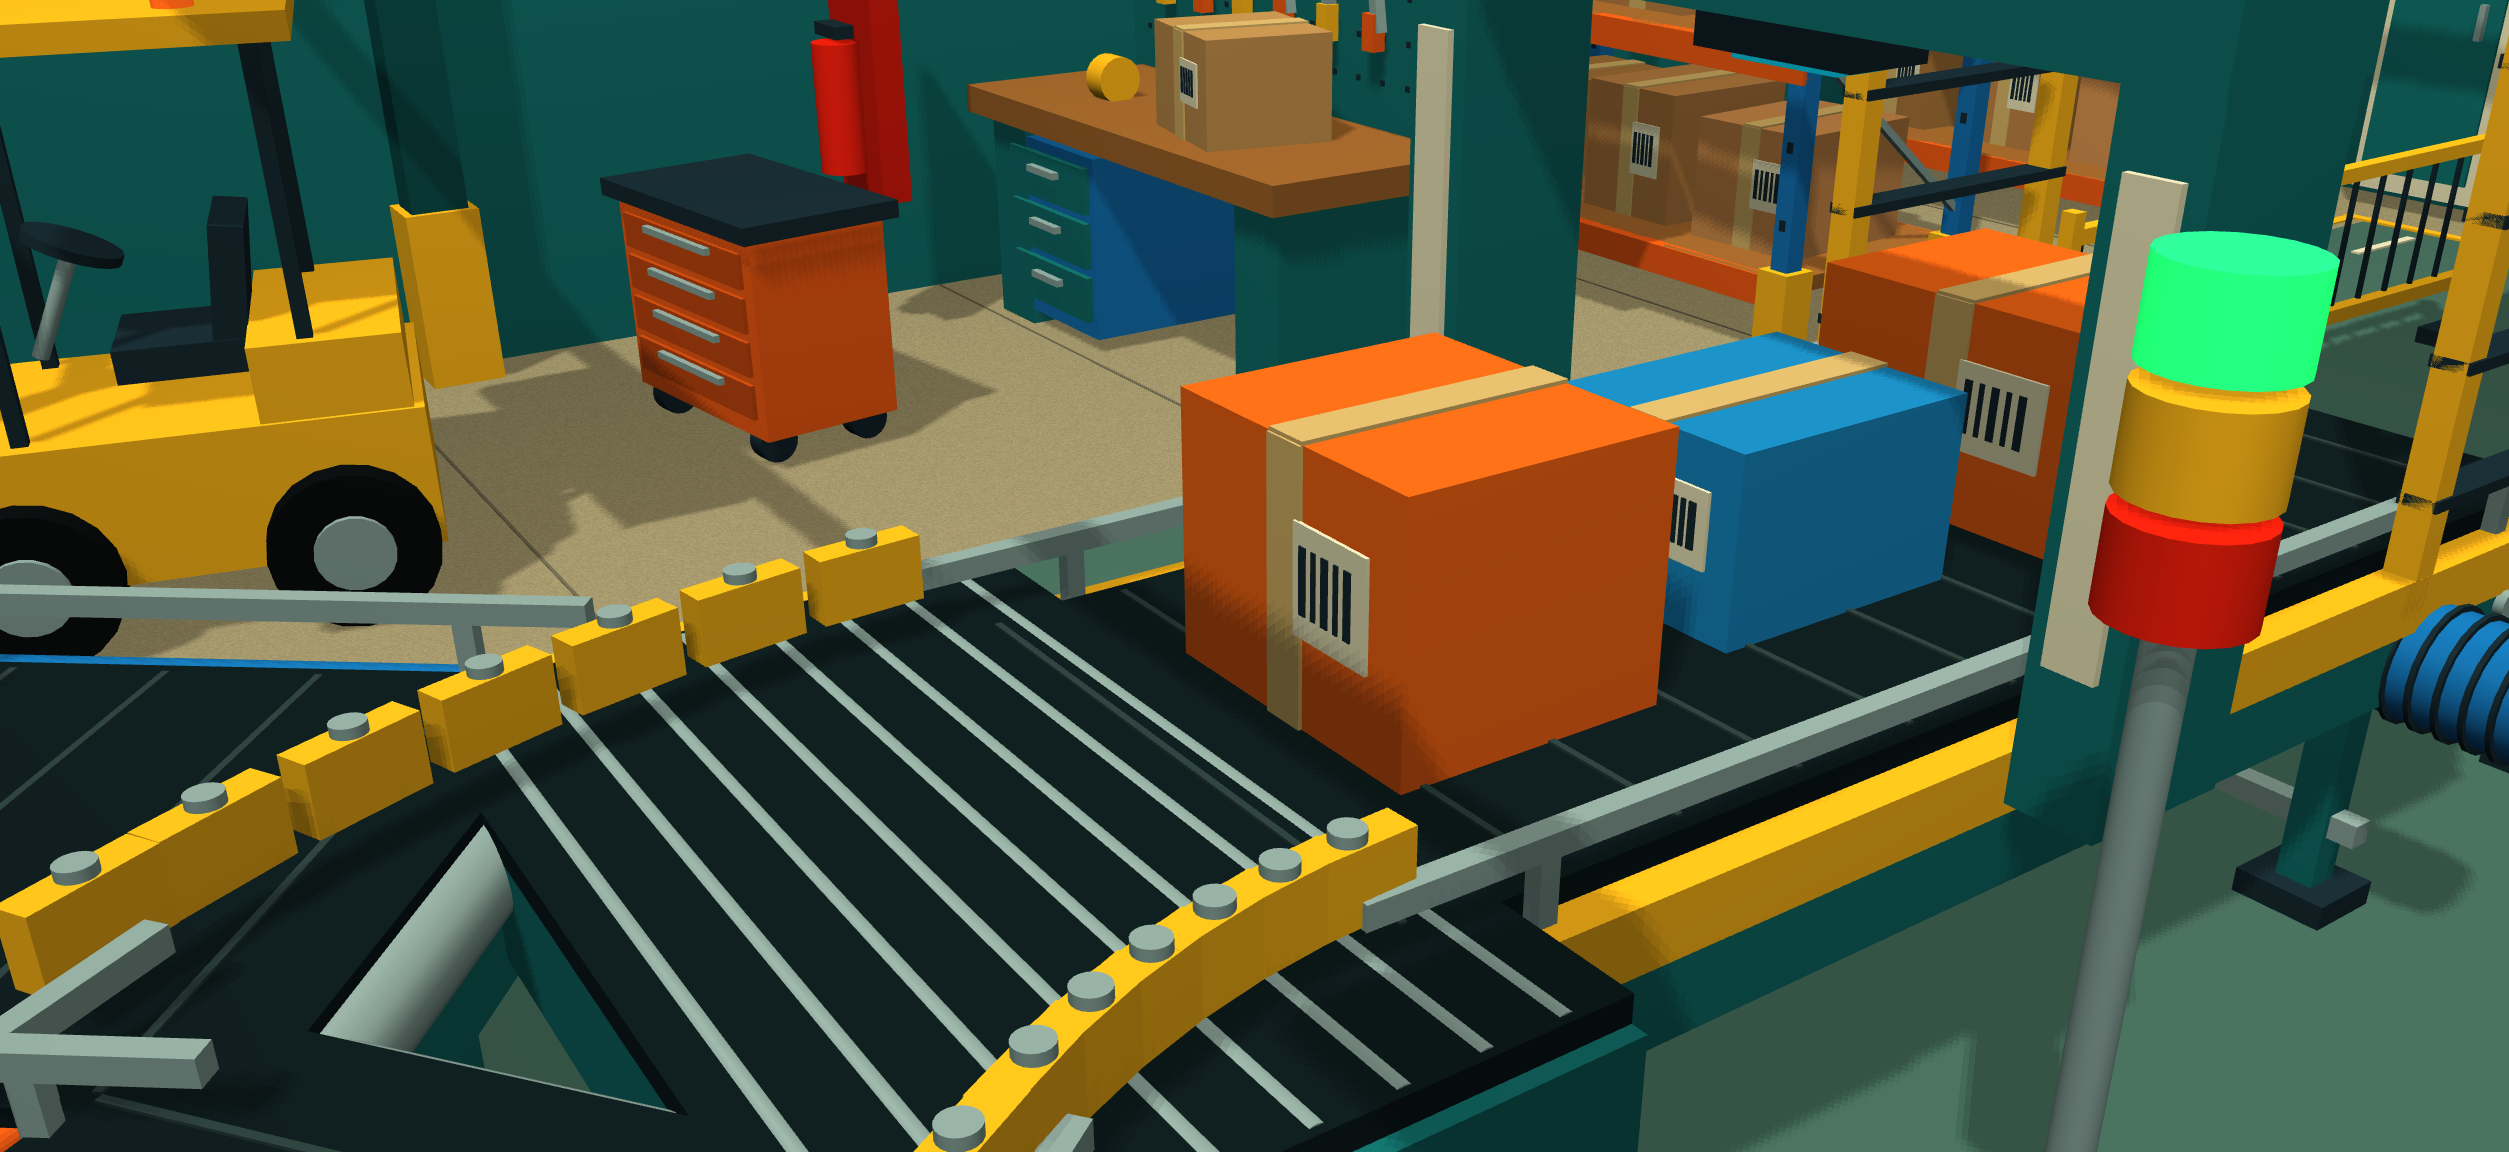
\includegraphics[width=\linewidth]{assets/phong_detail_crop.png}\par\small\textbf{A. Phong shading:} lighting calculated at each fragment.\end{minipage}\hfill
\begin{minipage}{0.49\linewidth}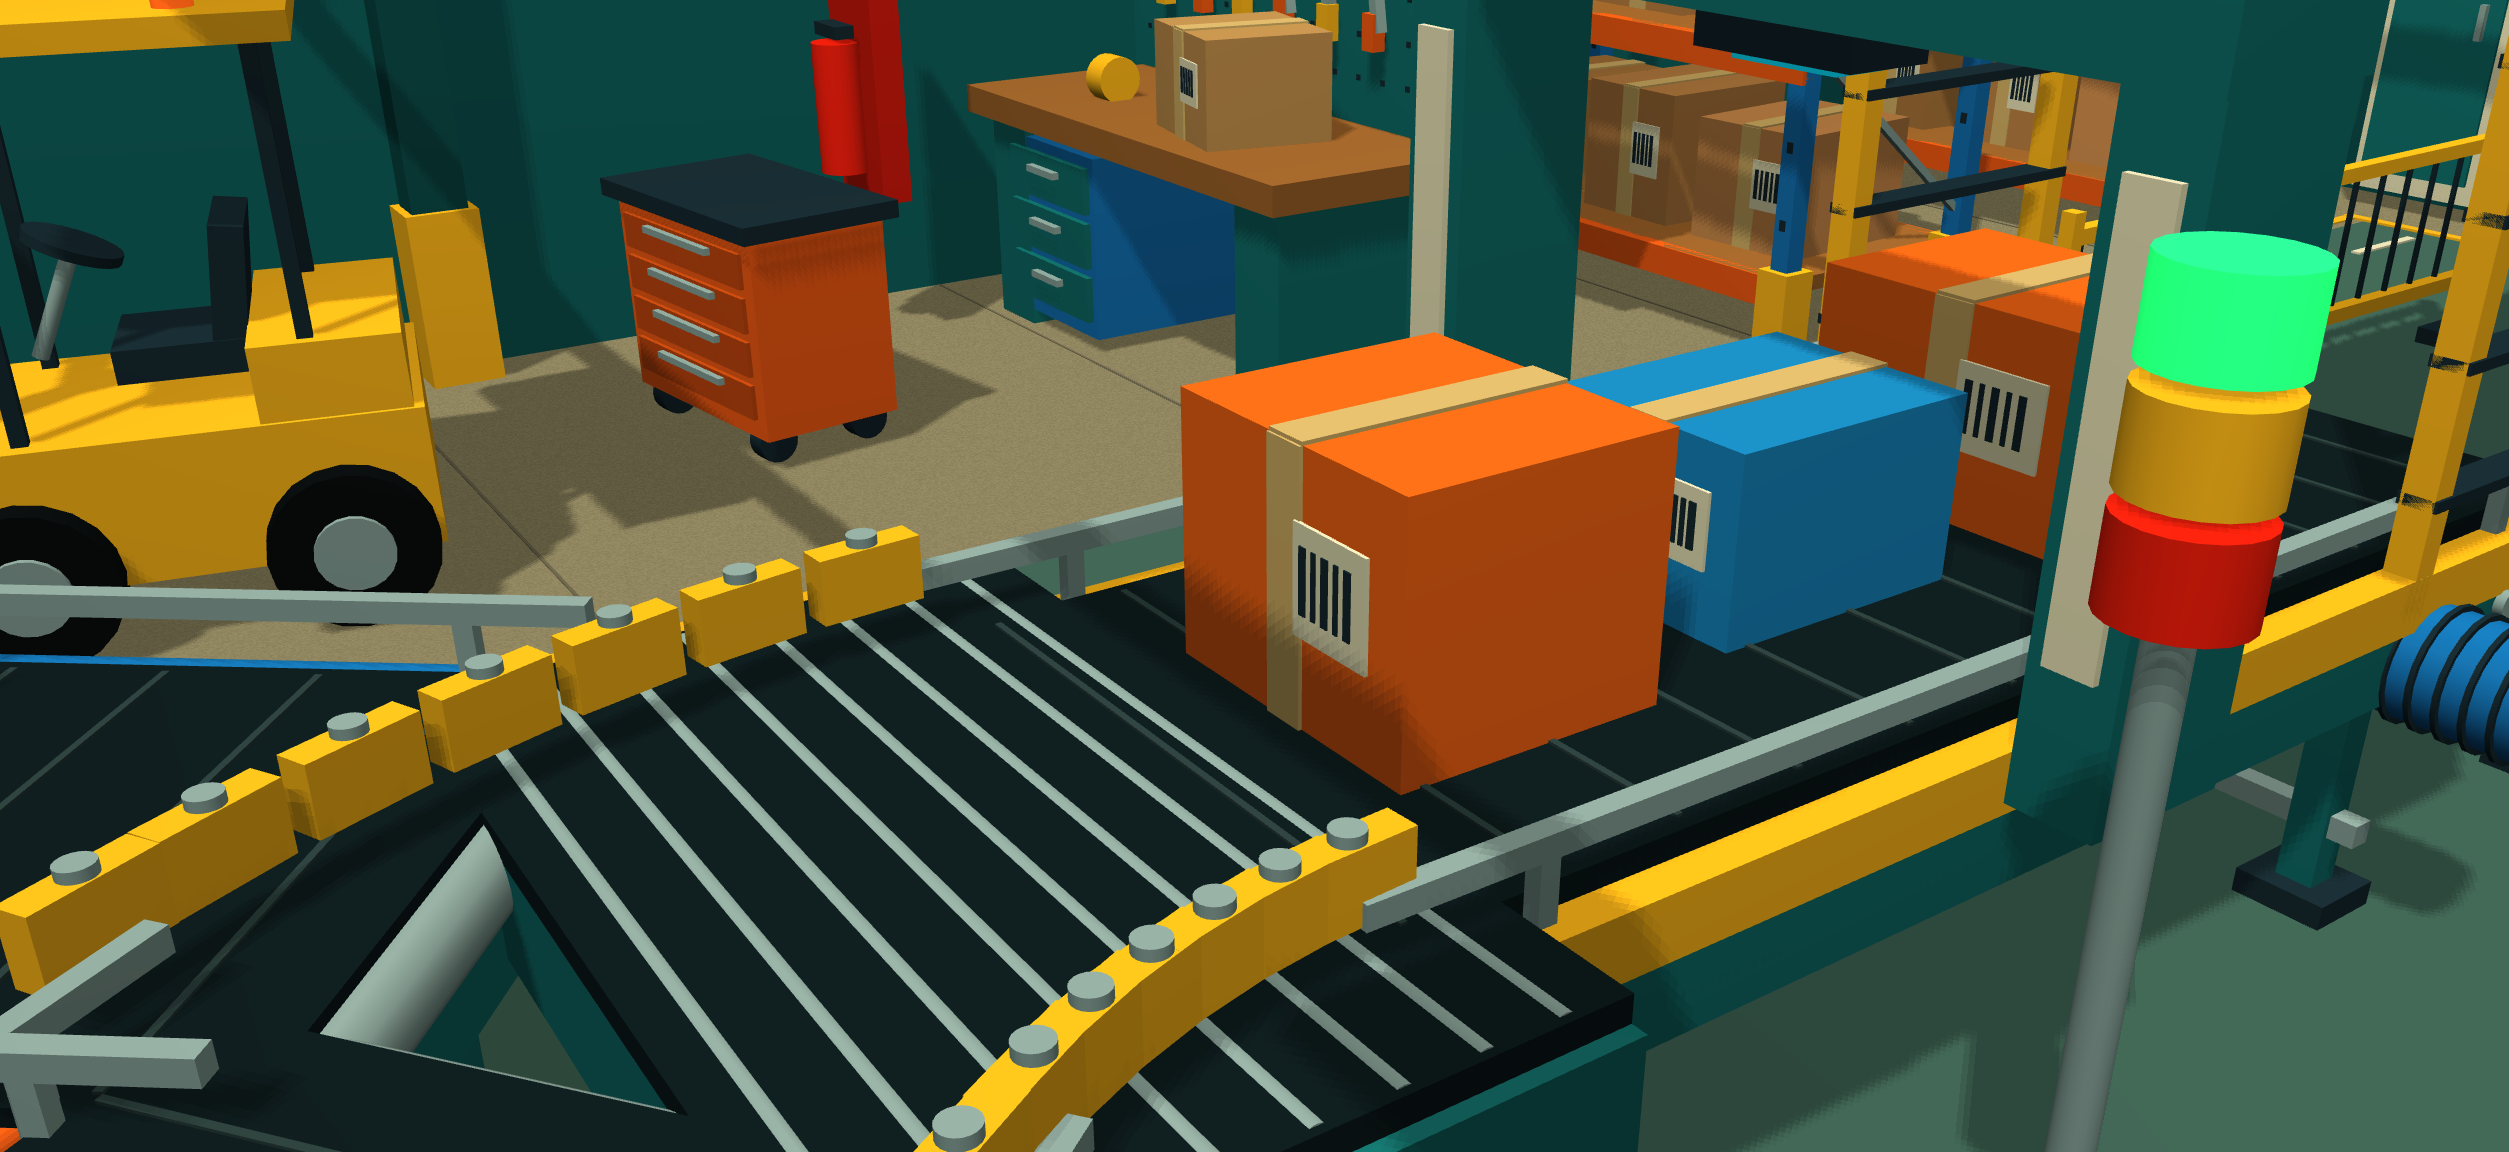
\includegraphics[width=\linewidth]{assets/gouraud_detail_crop.png}\par\small\textbf{B. Gouraud shading:} lighting calculated at vertices.\end{minipage}
\caption{Comparison at the same camera position and 24 s simulation time. Differences are most visible on the silver guides, rails and cylindrical roller; matte boxes show less variation.}
\end{figure}
\begin{shot}[0.85\linewidth]{assets/phong_detail_crop.png}{Detailed view of the default shading mode. Rail highlights and variations in face brightness provide depth cues.}
\callout{0.42,0.24}{0.17,0.12}{Metal highlights}
\callout{0.58,0.52}{0.80,0.80}{Matte box face}
\end{shot}
\subsection{Implemented illumination model}
Let $B$ be base RGB color, $C$ light color, $N$ the unit normal, $L$ the direction toward light, and $V$ the direction toward the camera. A dot product measures how closely directions align; RGB products act component by component.
\par{\small\begin{tabularx}{\textwidth}{@{}L{24mm}Y@{}}\toprule
\textbf{Term} & \textbf{Contribution and implemented equation}\\\midrule
Ambient & Provides background illumination. With $t=(N_y+1)/2$, $I_a=B[(1-t)(.20,.22,.21)+t(.48,.50,.47)]$.\\
Diffuse & Uses the Lambert cosine rule: $I_d=BC\max(N\cdot L,0)$.\\
Specular & Produces highlights. $H=\operatorname{normalize}(L+V)$; $u=\operatorname{clamp}((m-10)/70,0,1)$; $S=.22u^2(3-2u)\max(N\cdot H,0)^m$. Contribution is $SC$.\\\bottomrule
\end{tabularx}}\par
The default uses Phong shading with the Blinn-Phong specular term above. Parcels use shininess $m=8$ (no specular contribution); rollers use 90 and guides use 55. The key \code{P} switches to Gouraud shading. Shadows and emission are evaluated per fragment in both modes.

\subsection{Phong reflection and shading formulas}
For one light, the classic Phong reflection model is
\begin{equation}
I_{\mathrm{Phong}}=k_a I_A+k_d C\max(N\cdot L,0)
+k_s C\max(R\cdot V,0)^m,\qquad R=2(N\cdot L)N-L.
\end{equation}
Here $I_A$ is ambient illumination; $k_a$, $k_d$ and $k_s$ are ambient, diffuse and specular material coefficients; and $m$ is the shininess exponent. RGB multiplication is component-wise. The project uses $\max(N\cdot H,0)^m$ in place of $\max(R\cdot V,0)^m$ for its Blinn-Phong highlights.

Phong shading interpolates vertex normals and evaluates illumination at each fragment $p$:
\begin{equation}
N(p)=\operatorname{normalize}\!\left(\sum_{i=1}^{3}w_i(p)N_i\right),
\qquad I_P(p)=F\bigl(N(p),L(p),V(p)\bigr).
\end{equation}
The function $F$ denotes the illumination model, and $N_i$ are vertex normals. The interpolation weights $w_i(p)$ are corrected for perspective and satisfy $\sum_iw_i(p)=1$.

\subsection{Gouraud shading formula}
Gouraud shading evaluates illumination at the three vertices and interpolates the resulting colors:
\begin{equation}
I_i=F(N_i,L_i,V_i),\qquad
I_G(p)=\sum_{i=1}^{3}w_i(p)I_i.
\end{equation}
Both modes use the same implemented illumination model. Gouraud shading may miss a small highlight inside a triangle when it is absent at all three vertices.
\source{\code{basic.frag}: \code{phong()}; \code{basic.vert}: \code{lightingAtVertex()}.}

\clearpage
\section{Lights, shadows and surface detail}
\label{sec:lights}
\begin{figure}[H]\centering
\begin{minipage}{0.49\linewidth}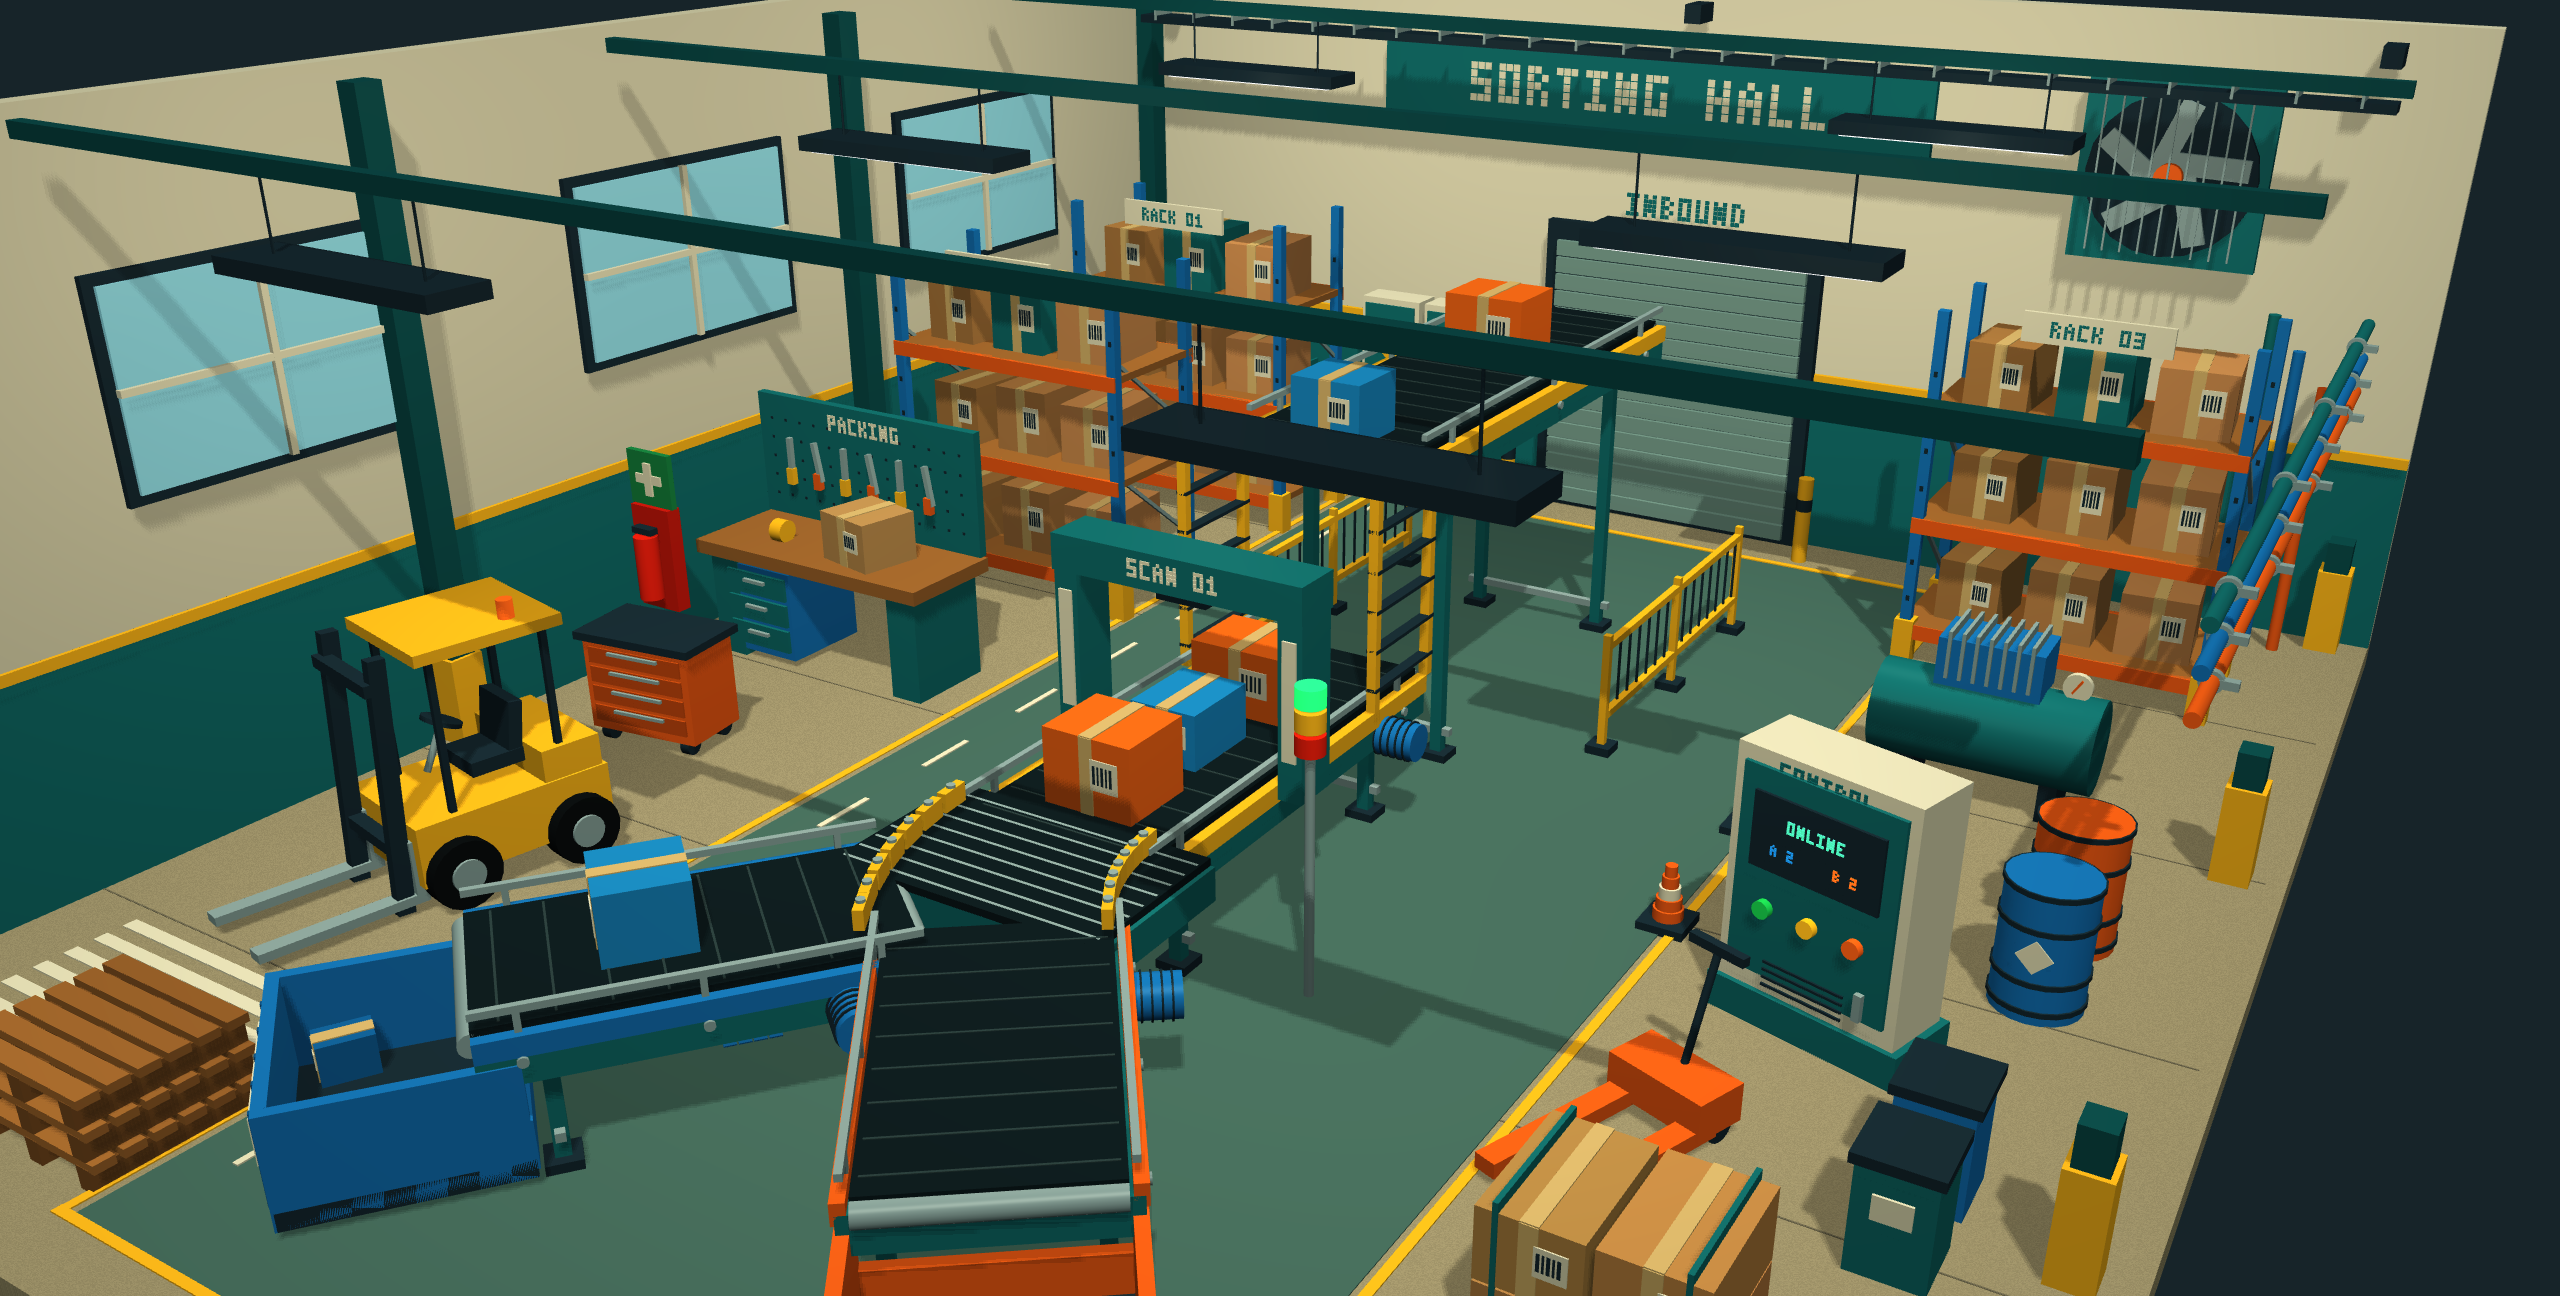
\includegraphics[width=\linewidth]{assets/lights_on_crop.png}\par\small\textbf{A. Point lights on:} warmer, brighter surfaces.\end{minipage}\hfill
\begin{minipage}{0.49\linewidth}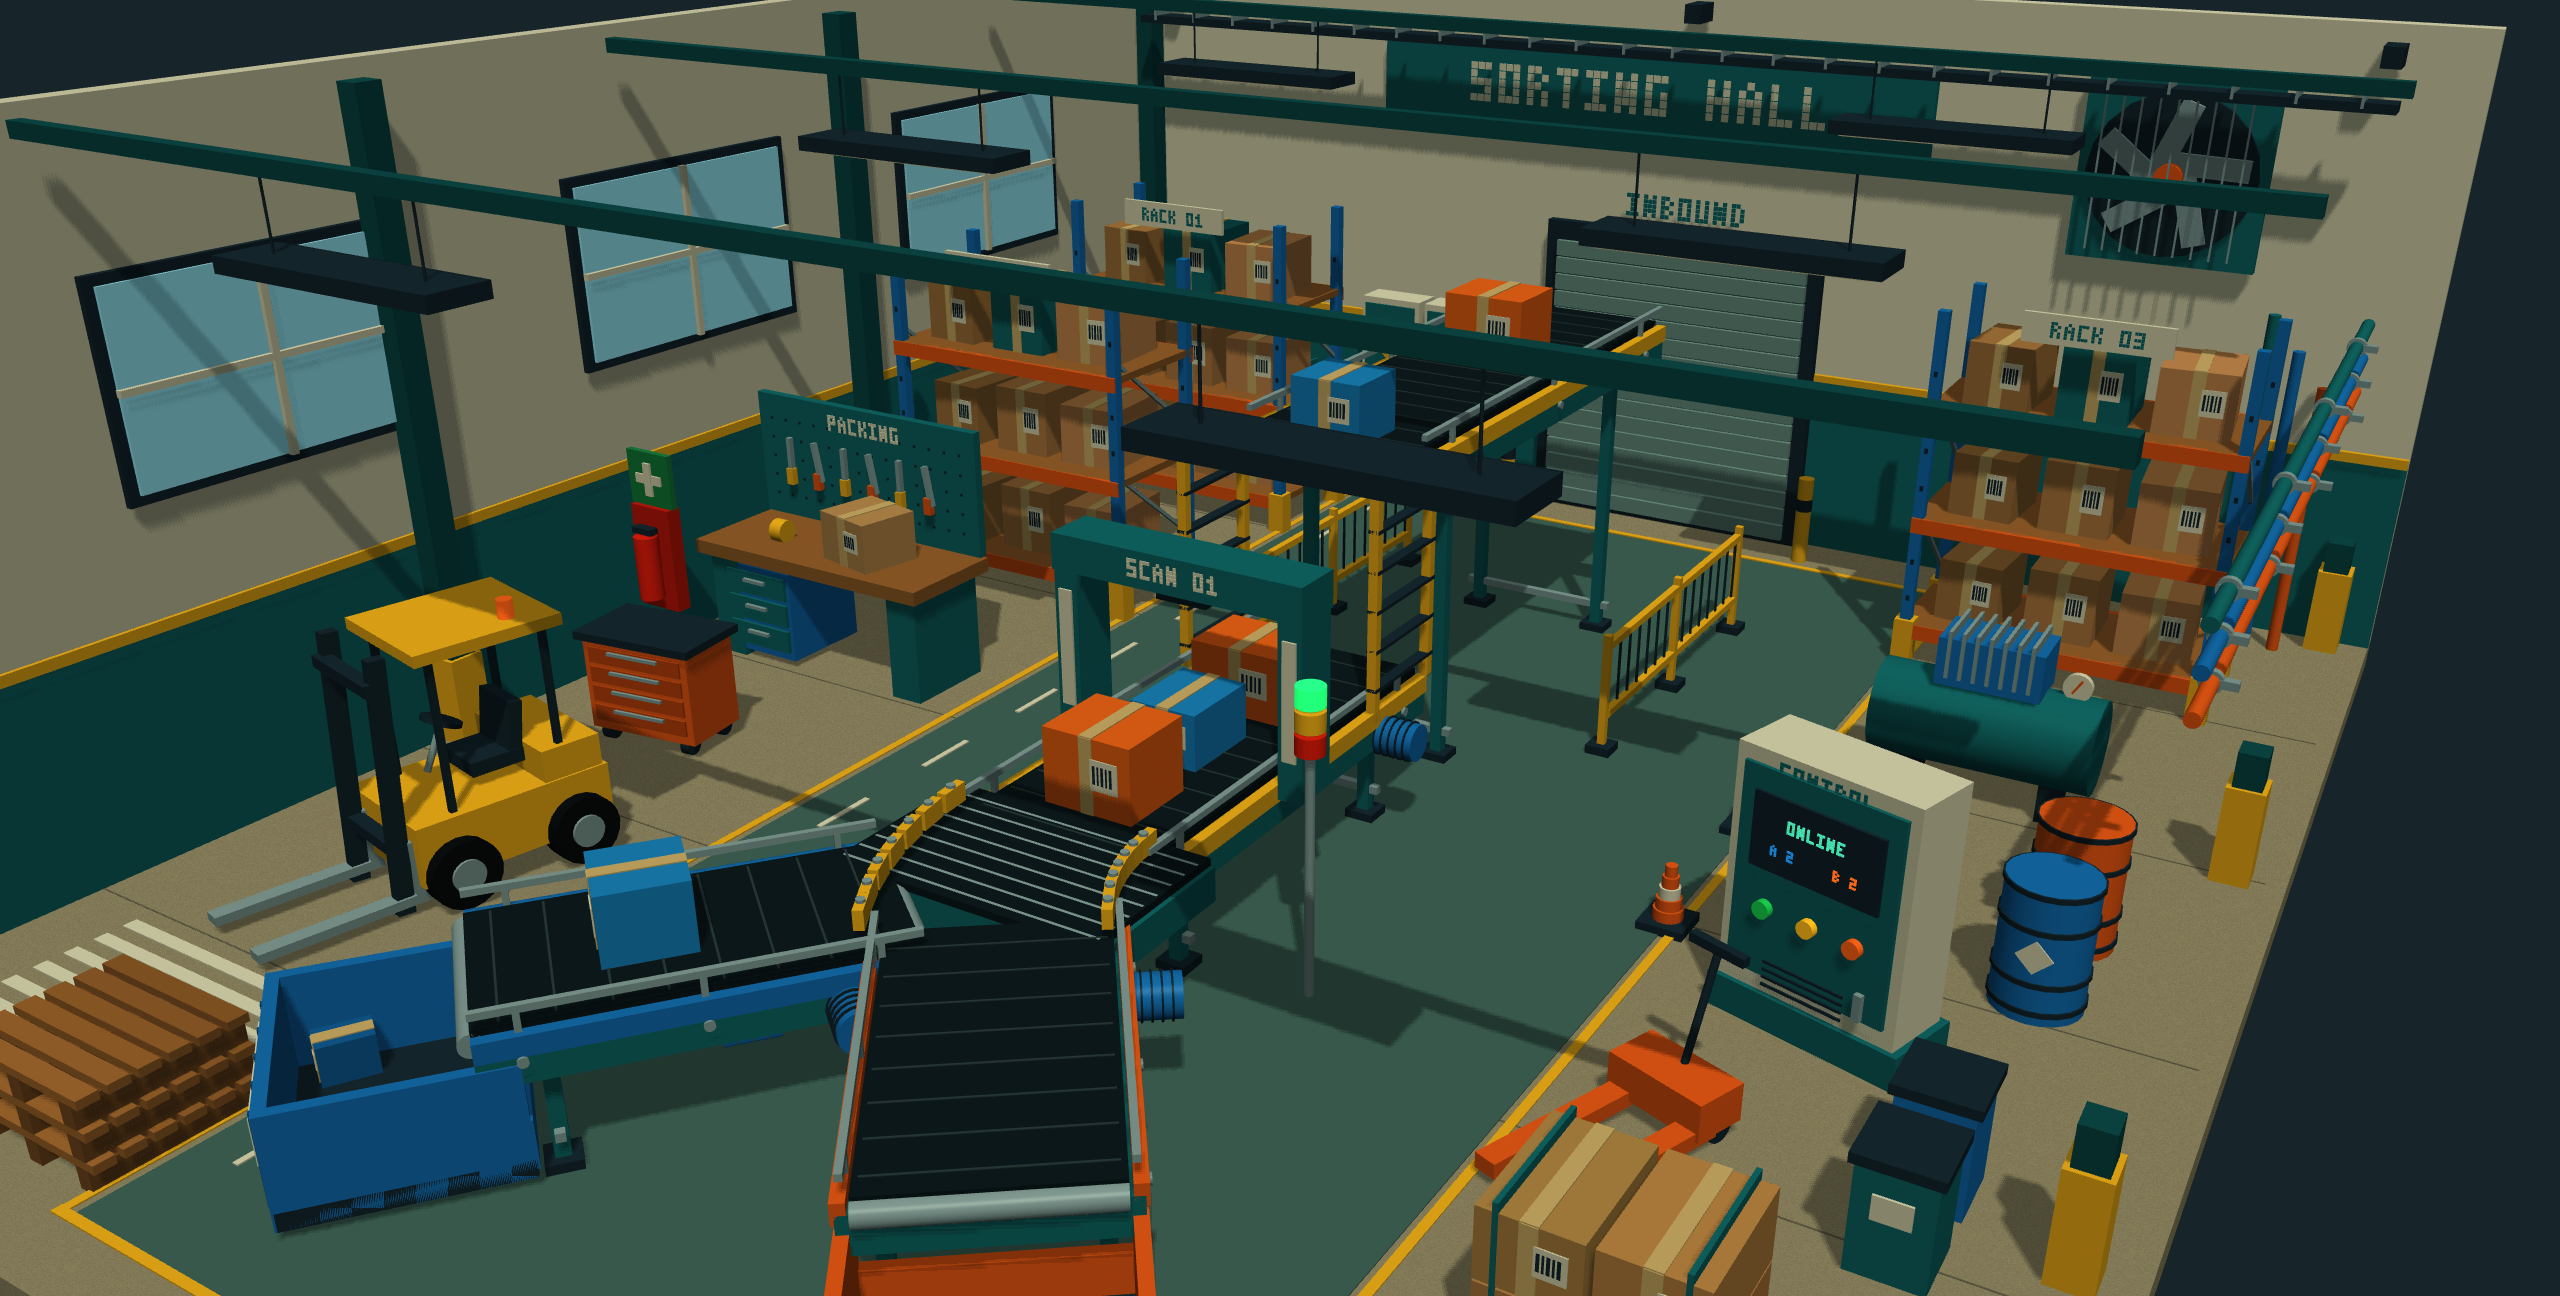
\includegraphics[width=\linewidth]{assets/lights_off_crop.png}\par\small\textbf{B. Point lights off:} ambient and daylight remain.\end{minipage}
\caption{Matched 24 s frames show the effect of the \code{L} toggle. No exposure or color adjustment was applied.}
\end{figure}
\begin{shot}{assets/shadow_detail.png}{Floor and machine detail cropped from the actual rendering. Shadows anchor objects to the floor; repeated markings define the work area.}
\callout{0.60,0.78}{0.18,0.82}{Floor shadow}
\callout{0.66,0.66}{0.78,0.12}{Safety border}
\end{shot}
\subsection{Lighting and surface models}
\textbf{Point lights:} four warm lights at $(\pm4.8,6.75,-6)$ and $(\pm4.8,6.75,5)$ use distance attenuation
\begin{equation}
A(d)=\frac{1}{1+0.025d+0.012d^2}.
\end{equation}
Their combined contribution is $0.36\sum A(d_i)F_i$, where $F_i$ contains diffuse and specular light. Daylight points toward $(10,24,14)$.

\textbf{Shadows:} a 2048 by 2048 light-view depth map stores the nearest surface. The camera pass compares its depth against nine neighboring samples (3 by 3 PCF). Shadow fraction $q=n_{blocked}/9$ reduces daylight by $1-0.78q$. A small depth bias prevents false self-shadows; point lights do not cast shadows.

\textbf{Emission:} $eB$ brightens lamps, scan lines and text. It has no bloom or nearby illumination. \textbf{Floor grain:} $c=\lfloor95(p_x,p_z)\rfloor$, $g=\operatorname{fract}(\sin(c\cdot(12.9898,78.233))43758.5453)$ and $f=0.95+0.10g$ slightly vary floor color. No image texture is loaded.

The shader adds ambient, shadowed daylight, enabled point lights and emission, then applies color rolloff $C_{out}=C_{pre}/(1+0.22C_{pre})$. Output is opaque; there is no gamma-correction stage.
\source{\code{main.cpp}: light uniforms and shadow passes; \code{basic.frag}: \code{shadowAmount()}, floor grain, emission and final color.}

\clearpage
\section{Controls, status and camera views}
\label{sec:controls}
\begin{figure}[H]\centering
\begin{minipage}{0.54\linewidth}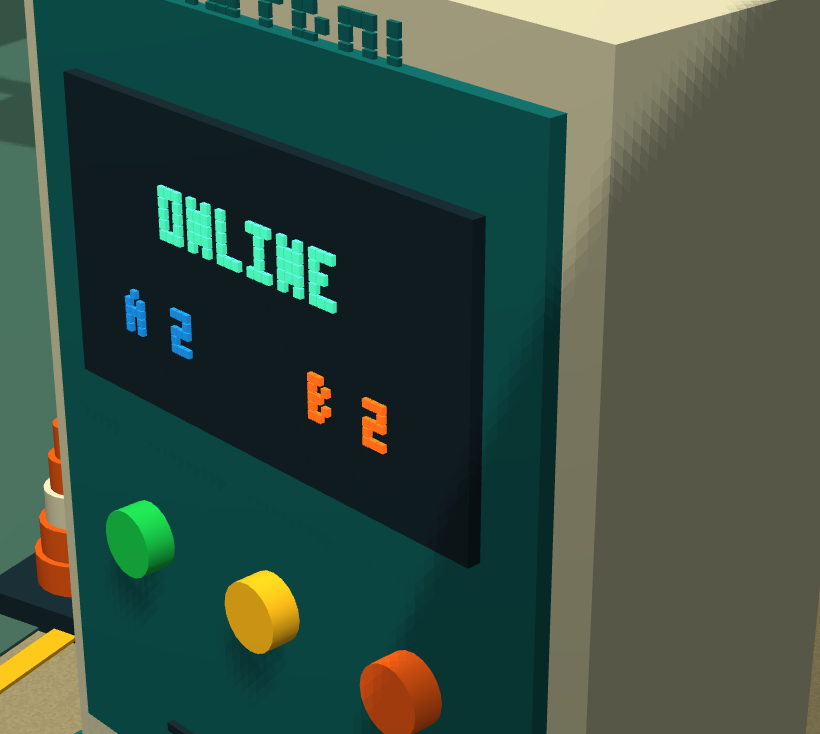
\includegraphics[width=\linewidth,height=55mm,keepaspectratio]{assets/cabinet_crop.png}\par\small\textbf{Cabinet at 24 s:} ONLINE, A = 2, B = 2. The modeled buttons are decorative.\end{minipage}\hfill
\begin{minipage}{0.42\linewidth}\small
\textbf{System status}\par
The cabinet shows running/paused and two collection counts. The tower shows the current operating stage. Brightness is emission: active 1.00, inactive 0.03.
\end{minipage}
\caption{Close-up of the actual status display and its geometric lettering.}
\end{figure}
\begin{figure}[H]\centering
\begin{minipage}{0.31\linewidth}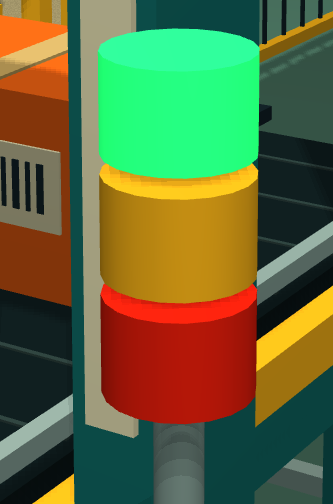
\includegraphics[width=\linewidth,height=34mm,keepaspectratio]{assets/tower_run_crop.png}\par\small\textbf{Green: running.}\end{minipage}\hfill
\begin{minipage}{0.31\linewidth}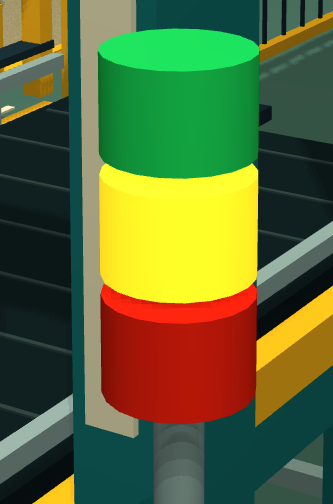
\includegraphics[width=\linewidth,height=34mm,keepaspectratio]{assets/tower_scan_crop.png}\par\small\textbf{Yellow: scanning.}\end{minipage}\hfill
\begin{minipage}{0.31\linewidth}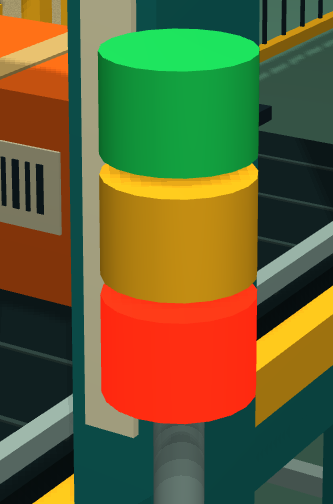
\includegraphics[width=\linewidth,height=34mm,keepaspectratio]{assets/tower_pause_crop.png}\par\small\textbf{Red: paused.}\end{minipage}
\caption{Same tower view, cropped equally. Run/pause are at 24 s; scanning is at 6.70 s.}
\end{figure}
\par{\small\begin{tabularx}{\textwidth}{@{}L{35mm}Y@{}}\toprule
\textbf{Input} & \textbf{Action}\\\midrule
\code{Space}; \code{+/-} & Pause/resume; change conveyor speed. Fan and camera continue during pause.\\
\code{G}; \code{L}; \code{P} & Request gate test; toggle point lights; switch Phong/Gouraud.\\
\code{R} & Reset parcels, counts, timers and angles; speed 1.55; resume. Camera/shading/light choice stay unchanged.\\
\code{1 / 2 / 3} & Overview / top / side camera presets.\\
\code{W A S D}; \code{Q/E} & Move camera forward/left/back/right; down/up at 8 units/s.\\
Mouse; wheel & Look around; zoom between $25^\circ$ and $70^\circ$ field of view.\\
\code{Tab}; click; \code{F11}; \code{Esc} & Release/recapture mouse; display mode; exit.\\\bottomrule
\end{tabularx}}\par
\subsection{Camera model and overhead view}
\begin{shot}{assets/top_layout.png}{Overhead factory view at 24 s. The upper and lower conveyors, scanner and branching exits define the sorting path.}
\callout{0.19,0.50}{0.18,0.85}{Entry conveyor}
\callout{0.54,0.51}{0.79,0.50}{Scanner}
\callout{0.68,0.50}{0.19,0.35}{Two-way sorter}
\end{shot}
\textbf{Camera implementation:} \code{glm::lookAt} constructs the view matrix. Perspective uses a $50^\circ$ default field of view, aspect ratio $W/H$, near plane 0.1 and far plane 100. Vertex position is $PVMp$. The top preset also uses perspective projection. Walls near the camera are omitted; at camera height 20 or above, beam and lamp meshes are omitted to reveal the conveyor layout. These rules also affect the shadow pass.
\source{\code{Camera.cpp}; \code{main.cpp}: callbacks and camera projection; \code{FactoryScene.cpp}: cabinet, tower and cutaway.}

\end{document}
